%\documentclass[iop]{emulateapj}
\documentclass[preprint]{aastex}
%\documentclass[12pt, onecolumn]{emulateapj}
%\documentstyle[aas2pp4,natbib209]{article}

\usepackage{tikz}
\usepackage{natbib}
\usepackage{amsmath}

\usetikzlibrary{shapes.geometric, arrows}
\usetikzlibrary{fit}

\tikzstyle{hyper} = [circle, text centered, draw=black]
\tikzstyle{param} = [circle, text centered, draw=black]
\tikzstyle{data} = [circle, text centered, draw=black, line width=2pt]
\tikzstyle{arrow} = [thick,->,>=stealth]

\newcommand{\myemail}{aimalz@nyu.edu}
\newcommand{\textul}{\underline}

\shorttitle{Galaxy population statistics from redshift distribution functions}
\shortauthors{Malz and Hogg}

\begin{document}

\title{Inference of galaxy population statistics given photometric redshift 
probability distribution functions}

\author{A.I. Malz\altaffilmark{1} \& David W. Hogg\altaffilmark{1,2,3,4}}
\email{aimalz@nyu.edu}

\altaffiltext{1}{Center for Cosmology and Particle Physics, Department of 
Physics,
  New York University, 4 Washington Pl., room 424, New York, NY 10003, USA}
\altaffiltext{2}{Simons Center for Data Analysis, 160 Fifth Avenue, 7th floor, 
New York, NY 10010, USA}
\altaffiltext{3}{Center for Data Science, New York University, 726 Broadway, 
7th floor, New York, NY 10003, USA}
\altaffiltext{4}{Max-Planck-Institut f\"ur Astronomie, K\"onigstuhl 17, D-69117 
Heidelberg, Germany}

\begin{abstract}
Ongoing and upcoming galaxy surveys aiming to constrain cosmological parameters 
will produce photometric redshift (photo-$z$) probability distribution 
functions (PDFs), which are, presumably, posteriors under some interim prior.  
We present a fully probabilistic approach to obtain the posterior distribution 
on a one-point statistic from a survey providing photo-$z$ interim posteriors 
and their interim prior.  The technique uses a probabilistic graphical model 
corresponding to the hierarchical Bayesian relation of photo-$z$ PDFs to a 
posterior distribution over the one-point statistic.  This mathematically 
consistent method is applied to the redshift distribution function $N(z)$ 
necessary for the calculation of cosmological parameters from weak lensing 
surveys, validated on synthetic data, and tested on a small subset of BOSS DR10 
data.  It is demonstrated that this method improves accuracy, both 
qualitatively and as quantified by the Kullback-Leibler Divergence, compared to 
popular alternatives (such as stacking of photo-$z$ PDFs and conversion of 
photo-$z$ PDFs to point estimates).  The method can be straightforwardly 
generalized to other one-point statistics including distribution functions over 
luminosity, mass, star formation rate, etc.
\end{abstract}

\keywords{methods: analytical "\_\_\_" methods: data analysis "\_\_\_" methods: 
statistical "\_\_\_" techniques: photometric "\_\_\_" galaxies: statistics, }

%\clearpage
\section{Introduction}
\label{sec:intro}

Photometric redshift (photo-$z$) estimation has been a staple of studies of 
galaxy evolution, large-scale structure, and cosmology since its conception 
decades ago \citep{Baum1962}.  An extremely coarse spectrum in the form of 
photometry in a handful of broadband filters can be an effective substitute for 
the time-intensive process of obtaining a spectroscopic redshift (spec-$z$), a 
procedure that may only be applied to relatively bright galaxies.  Once the 
photometric colors are calibrated against either a library of spectral energy 
distribution (SED) templates or a data set of spectra for galaxies with known 
redshifts, a correspondence between photometric colors and redshifts may be 
constructed, forming a trustworthy basis for photo-$z$ estimation or testing.

Many more photo-$z$s may be obtained in the time it would take to observe a 
smaller number of spec-$z$s, and photo-$z$s may be measured for galaxies too 
dim for accurate spec-$z$ confirmation, permitting the compilation of large 
surveys of galaxy redshifts spanning a broad range of redshifts and 
luminosities.  Photo-$z$s have thus enabled the era of precision cosmology, 
heralded by weak gravitational lensing tomography and baryon acoustic 
oscillation peak measurements.  Calculations of correlation functions of cosmic 
shears and galaxy positions require large numbers of high-confidence redshifts 
of surveyed galaxies.  

However, photo-$z$s are susceptible to a number of sources of error, 
particularly their inherent noisiness due to the coarseness of photometric 
filters, catastrophic errors in which galaxies of one type at one redshift are 
mistaken for galaxies of another type at a different redshift, and systematics 
introduced by observational techniques, data reduction processes, and training 
set limitations.  In addition to these limitations in accuracy, there is also 
the matter of precision; photo-$z$s are often reported with error bars derived 
without inclusion of all systematic errors, including the different selection 
effects between the photometric color- or magnitude-spaces of galaxies for 
which photo-$z$s are desired and galaxies with spec-$z$s used to calibrate 
photo-$z$ estimators.

Once propagated through the calculations of correlation functions of cosmic 
shear and galaxy positions, these sources of photo-$z$ errors are not 
insignificant contributors to the total uncertainties reported on cosmological 
parameters; as other systematic errors have been resolved, the uncertainties 
associated with photo-$z$s have come to dominate the uncertainties on estimates 
of cosmological parameters made by current surveys such as CFHTLens and DES.

Much effort has been dedicated to improving photo-$z$s, though they are still 
most commonly obtained by a maximum likelihood estimator (MLE) based on 
libraries of galaxy spectral energy distribution (SED) templates, with 
conservative approaches to error estimation.  Recent advances have focused on 
identifying and removing catastrophic outliers when using photo-$z$s for 
inference \citep{Gorecki2014}.  Sophisticated Bayesian techniques and 
cutting-edge machine learning methods have been employed to improve precision 
\citep{Carliles2010} and accuracy \citep{Sadeh2015}. 

An alternative to point estimation of photo-$z$s is redshift probability 
distribution function (PDF) estimation, in which rather than an MLE point 
estimate, the full posterior (or likelihood) PDF of the redshift of a galaxy is 
reported \citep{Koo1999}.  This option is favorable because it contains more 
potentially useful information than a point estimate while addressing the 
issues with precision, accuracy, and systematics.  Photo-$z$ PDFs are not 
without their own weaknesses, including the resources necessary to calculate 
and record them for large galaxy surveys \citep{CarrascoKind2014} and the 
method used to derive them.  The most important of these issues, however, is 
that use of them in the literature is inconsistent at best and incorrect at 
worst.  This paper aims to develop a clear methodology guiding the use of 
photo-$z$ PDFs in inference so they may best be utilized by the community.

Many techniques to obtain photo-$z$ probability distributions have been 
proposed and tested in the literature.  An extension of the Bayesian 
photometric redshift (BPZ) method of \citet{Benitez2000} that produces 
posterior probability distributions (as opposed to a selection of local maxima) 
from an SED template library has been employed \citep{Hildebrandt2012, 
Kelly2014, Lopez-Sanjuan2015}.  Photo-$z$ posterior probability distributions 
have also been obtained by a variety of trustworthy data-driven approaches in 
the literature: $k$-nearest neighbor algorithms with \citep{Ball2008} and 
without \citep{Sheldon2012} inclusion of photometric measurement errors, neural 
networks \citep{Bonnett2015a}, self-organizing maps \citep{CarrascoKind2014a}, 
and prediction tree and random forest classification techniques 
\citep{Carliles2010, CarrascoKind2013}.  (The approaches of fitting to a 
training set and fitting to a template library are related by 
\citet{Budavari2009}.)  Hierarchical inference has also been applied to 
calculate photo-$z$ posteriors simultaneously with the overall redshift 
distribution function \citep{Leistedt2016}.  Some current work aims to vet 
photo-$z$ probability distribution generation methods \citep{Wittman2016}, but 
much remains to be done.  Of course, this brief review does not cover all ways 
to obtain photo-$z$ probability distribution functions; many more may be found 
in the literature, along with comparisons thereof \citep{Hildebrandt2010, 
Dahlen2013, Sanchez2013, Bonnett2015}.

Photo-$z$ probability distributions have been produced by completed surveys 
\citep{Hildebrandt2012, Sheldon2012} and will be produced by ongoing and 
upcoming surveys \citep{LSSTScienceCollaboration2009, CarrascoKind2014a, 
Bonnett2015, Masters2015}.  Though their potential to improve estimates of 
physical parameters is tremendous, photo-$z$ posterior probability 
distributions have been applied only to a limited extent.  They have been used 
to form selection criteria of samples from galaxy surveys without propagation 
through the calculations of physical parameters 
\citep{VanBreukelen2009,Viironen2015}.  Probability cuts on Bayesian quantities 
are not uncommon \citep{Leung2015, DiPompeo2015a}, but that procedure does not 
fully take advantage of all information contained in a probability distribution 
for parameter inference.  

Despite the growing prevalence of photo-$z$ posterior production, no 
implementation of inference using photo-$z$ PDFs has yet been presented with a 
mathematically consistent methodology.  We present and validate a technique for 
the use of photo-$z$ posterior distributions in inference of arbitrary 
statistics relevant to cosmology, large-scale structure, and galaxy evolution.  
For simplicity, we consider only one-point statistics, though future work will 
extend this methodology to higher-order statistics.

The redshift distribution function $N(z)$ serves as an ideal statistic upon 
which to demonstrate this novel approach.  $N(z)$ is necessary for calculations 
of two-point correlation functions of weak gravitational lensing and counting 
statistics that are used to probe dark energy \citep{Masters2015}.  $N(z)$ for 
observed galaxies has also been used to validate survey selection functions 
used in generation of realistic, multi-purpose mock catalogs 
\citep{Norberg2002}.  Additionally, $N(z)$ has been the subject of inference 
using photo-$z$ probability distributions before \citep{Sheldon2012, 
Hildebrandt2012, Kelly2014, Benjamin2013, Bonnett2015a, Viironen2015, 
Asorey2016, Leistedt2016}, so comparisons to the literature may easily be made. 
 

\textbf{New paragraph here: Say what precision is needed for N(z) for future 
weak lensing surveys. Say what precision the mass function is needed (in, say 
cluster studies) for precision cosmology; that's also relevant in principle}

Sec. \ref{sec:meth} will derive the framework for exploring the full posterior 
of distribution for $N(z)$ using photo-$z$ probability distribution functions.  
Sec. \ref{sec:exp} will describe how the model given in Sec. \ref{sec:meth} is 
implemented.  Sec. \ref{sec:valid} will discuss the results of applying the 
fully probabilistic approach to mock and real datasets.

%\clearpage
\section{Method}
\label{sec:meth}

Consider a survey of $J$ galaxies $j$, each with photometric data 
$\vec{d}_{j}$; thus the entire survey over some solid angle $\Omega$ produces 
the ensemble of photometric magnitudes (or colors) and their associated 
observational errors $\{\vec{d}_{j}\}$.  Each galaxy $j$ has a redshift $z_{j}$ 
that we would like to learn; redshift is a parameter in this case.  The 
distribution of the ensemble of redshifts $\{z_{j}\}$ may be described by the 
hyperparameters defining the redshift distribution function $N(z)$ that we 
would like to quantify.  This situation may be considered to be a probabilistic 
generative model, illustrated by the directed acyclic graph of Fig. 
\ref{fig:flow}.  

\begin{figure}
\vspace{0.5cm}
\begin{center}
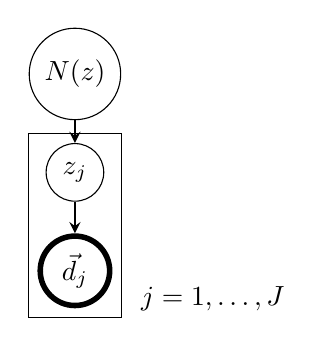
\begin{tikzpicture}[node distance=1cm]

\node (nz) [hyper] {$N(z)$};
\node (z) [param, below of=nz,yshift=-0.25cm] {$z_{j}$};
\node (mags) [data, below of=z,yshift=-0.25cm] {$\vec{d}_{j}$};
\node (survey) [draw=black,fit={(mags.west)(z.north)(mags.south)(mags.east)}] 
{};
\node [xshift=1.75cm,yshift=0.25cm] at (survey.south) {$j=1,\dots,J$};

\draw [arrow] (nz) -- (z);
\draw [arrow] (z) -- (mags);

\end{tikzpicture}
\caption{This directed acyclic graph illustrates the hierarchical model 
presented in this paper.  The redshift distribution function $N(z)$ exists 
independent of the survey of $J$ galaxies, indicated as a box.  The redshifts 
$\{z_{j}\}$ of all galaxies in the survey are parameters independently drawn 
from $N(z)$.  The photometric data $\vec{d}_{j}$ encircled in bold are 
observable quantities determined by the corresponding galaxy's redshift 
$z_{j}$.  Because the data $\vec{d}_{j}$ of each galaxy can be used to infer 
its redshift $z_{j}$, $N(z)$ may be inferred from the collection of 
$\{\vec{d}_{j}\}$.}
\label{fig:flow}
\end{center}
\end{figure}

The redshift distribution function 
\begin{equation}
\label{eq:distribution}
N(z)=dN/dz
\end{equation}
 is the number of galaxies per unit redshift, effectively defining the 
evolution in the number of galaxies \citep{Menard2013}.  In the following 
sections, we will present and compare methods for calculating $N(z)$ from 
photometric redshift probability distribution functions.  Sec. \ref{sec:prob} 
contains the mathematical derivation of a probabilistic model for $N(z)$ 
dependent on photo-$z$ probability distribution functions, and Sec. 
\ref{sec:sheldon} contrasts the probabilistic model with alternative methods.

%\begin{eqnarray}
%\label{eq:distribution}
%N(z) &=& \frac{dN}{dz}
%\end{eqnarray}
%
%\clearpage
\subsection{Probabilistic Model Generalities}
\label{sec:prob}

We begin by parametrizing $N(z)$ in terms of $\vec{\theta}$, comprising some 
set of hyperparameters that define the form $N(z)$ may take in whatever basis 
we choose.  At this point, these hyperparameters are quite general and may 
represent coefficients in a high-order polynomial as a function of redshift, a 
set of means and variances defining Gaussians that sum to the desired 
distribution, a set of histogram heights that describe a binned version of the 
redshift distribution function, etc.  We define a function 
$f_{\vec{\theta}}(z)=N(z)$ that transforms these hyperparameters into the 
redshift distribution function $N(z)$.  Because 
\begin{equation}
\label{eq:definition}
N(z)\propto p(z|\vec{\theta}),
\end{equation}
we may discontinue discussion of $N(z)$ in favor of the likelihood 
$p(z|\vec{\theta})$.

In this paper, we shall work exclusively with log-probabilities.  What we wish 
to estimate is the full log-posterior probability distribution (hereafter the 
full log-posterior) of the hyperparameters $\vec{\theta}$ given the data 
$\{\vec{d}_{j}\}$.  By Bayes' Rule, the full log-posterior 
$\ln[p(\vec{\theta}|\{\vec{d}_{j}\})]$ may be expressed in terms of the full 
log-likelihood probability distribution (hereafter the full log-likelihood) 
$\ln[p(\{\vec{d}_{j}\}|\vec{\theta})]$ by way of a hyperprior log-probability 
distribution (hereafter the hyperprior) $\ln p(\vec{\theta})$ over the 
hyperparameters and the log-probability of the data $\ln[p(\{\vec{d}_{j}\})]$.  
The hyperprior expresses our beliefs about the distribution of the 
hyperparameters comprising $\vec{\theta}$.  This matter is a choice we cannot 
avoid making and one which is often inspired by the results of previous galaxy 
surveys.  The hyperprior chosen here will be elaborated upon in Sec. 
\ref{sec:exp}.

The full log-posterior can be probed with a quantity proportional to it so the 
log-probability of the data is never explicitly necessary.  The full 
log-likelihood may be expanded in terms of a marginalization over the redshifts 
as parameters, as in 
\begin{equation}
\label{eq:marginalize}
\ln[p(\{\vec{d}_{j}\}|\vec{\theta})] = \ln\left[\int\ 
p(\{\vec{d}_{j}\}|\{z_{j}\})\ p(\{z_{j}\}|\vec{\theta})\ d\{z_{j}\}\right].
\end{equation}

We shall make two assumptions of independence in order to make the problem 
tractable; their limitations are be discussed below.  First, we take 
$\ln[p(\{\vec{d}_{j}\}|\{z_{j}\})]$ to be the sum of $J$ individual 
log-likelihood distribution functions $\ln[p(\vec{d}_{j}|z_{j})]$, as in 
\begin{equation}
\label{eq:indiedat}
\ln[p(\{\vec{d}_{j}\}|\{z_{j}\})] = \sum_{j=1}^{J}\ \ln[p(\vec{d}_{j}|z_{j})],
\end{equation}
a result of the definition of probabilistic independence.  Second, we shall 
assume the true redshifts $\{z_{j}\}$ are $J$ independent draws from the true 
$p(z|\vec{\theta})$.  Additionally, $J$ itself is a Poisson random variable.  
The combination of these assumptions is given by 
\begin{equation}
\label{eq:indie}
\ln[p(\{z_{j}\}|\vec{\theta})] = -\int\ f_{\vec{\theta}}(z)\ dz +  
\sum_{j=1}^{J}\ \ln[p(z_{j}|\vec{\theta})].
\end{equation}
It is important to note that the integral $\int N(z)\ dz$ is not constrained to 
equal the variable defining the Poisson distribution but instead $J$ by 
(\ref{eq:definition}), which can be thought of as another parameter.  A 
detailed discussion of this matter may be found in \citet{Foreman-Mackey2014}.  
Applying Bayes' Rule, we may combine terms to obtain 
\begin{equation}
\label{eq:posterior}
\ln[p(\vec{\theta}|\{\vec{d}_{j}\})] \propto \ln[p(\vec{\theta})]\ -\int 
f_{\vec{\theta}}(z)\ dz + \sum_{j=1}^{J}\ \ln\left[\int\ p(\vec{d}_{j}|z_{j})\ 
p(z_{j}|\vec{\theta})\ dz_{j}\right].
\end{equation}

(\ref{eq:posterior}) contains two quantities that merit further discussion, the 
prior distribution $p(\vec{\theta})$ discussed further in Sec. \ref{sec:exp} 
and the photo-$z$ log-likelihoods $\ln[p(\vec{d}_{j}|z_{j})]$ that have not 
been mentioned since (\ref{eq:marginalize}).  Though photo-$z$ log-likelihoods 
would be desirable for use in these equations, they are not generally the 
product of either empirical and data-driven methods for obtaining photo-$z$ 
probability distributions.  Though probabilistic photo-$z$s are typically 
reported as generic probability distributions $p(z_{j})$, the methods that 
produce them may be understood to always yield posteriors, probability 
distributions conditioned on the data we believe to be true.  If they were not 
based in this assumption, they would require a sum over an infinite space of 
possible datasets.

Posteriors differ from likelihoods by way of a prior distribution, so we cannot 
simply assume that the available data products are photo-$z$ posteriors 
$p(z_{j}|\vec{d}_{j})$.  Rather, we consider the published catalog of 
$p(z_{j})$ interim photo-$z$ posteriors 
$p(z_{j}|\vec{d}_{j},\vec{\theta}^{*})$.  There must have been some interim 
prior probability distribution $p(z|\vec{\theta}^{*})$ defined in terms of the 
interim prior parameter values (hereafter the interim prior) $\vec{\theta}^{*}$ 
explicitly chosen or implicitly made to perform the calculation of the 
probabilistic photo-$z$s.  If it is implicit, it may not be representable in 
the parametrization we have chosen, and furthermore it may not be known at all; 
a method that produces interim photo-$z$ posteriors of this kind is not 
suitable for inference.  However, so long as the interim prior is known, 
hierarchical inference is possible. 

The interim prior $\vec{\theta}^{*}$ may be thought of as an initial guess for 
the parameters contained in $\vec{\theta}$, inspired by the generative model 
for photometry from the redshift distribution functions and including some 
parameters defining intrinsic galaxy spectra and instrumental effects. (See 
\citealt{Benitez2000} for more detail.)  For statistical purposes, we would 
like any interim prior to be uninformative, but this is rarely achievable.  In 
the case of estimating $N(z)$ photometrically, it is common to use 
$\vec{\theta}^{*}$ corresponding to $N(z)$ derived from some different, 
spectroscopically confirmed sample or from a cosmological simulation.

Since we only have access to interim photo-$z$ posteriors, we must be able to 
write the full log-posterior in terms of interim photo-$z$ log-posteriors 
rather than the log-likelihoods of (\ref{eq:posterior}).  However, we will need 
an explicit statement of this interim prior for whatever method is chosen to 
produce the interim photo-$z$ posteriors.  To perform the necessary 
transformation from likelihoods to posteriors, we follow the reasoning of 
\citet{Foreman-Mackey2014}.  Let us consider the probability of the parameters 
conditioned on the data and an interim prior and rewrite the problematic 
likelihood of (\ref{eq:posterior}) as 
\begin{equation}
\label{eq:trick}
p(\vec{d}_{j}|z_{j}) = p(\vec{d}_{j}|z_{j})\ 
\frac{p(z_{j}|\vec{d}_{j},\vec{\theta}^{*})}{p(z_{j}|\vec{d}_{j},\vec{\theta}^{*
})}.
\end{equation}

Once the interim prior $\vec{\theta}^{*}$ is explicitly introduced, we may 
expand the denominator according to Bayes' Rule to get 
\begin{equation}
\label{eq:expand}
p(\vec{d}_{j}|z_{j}) = p(\vec{d}_{j}|z_{j})\ 
p(z_{j}|\vec{d}_{j},\vec{\theta}^{*})\ 
\frac{p(\vec{d}_{j}|\vec{\theta}^{*})}{p(z_{j}|\vec{\theta}^{*})\ 
p(\vec{d}_{j}|z_{j},\vec{\theta}^{*})}.
\end{equation}
Because there is no direct dependence of the data upon the hyperparameters, we 
may again expand the term $p(\vec{d}_{j}|z_{j},\vec{\theta}^{*})$ to obtain 
\begin{equation}
\label{eq:indterm}
p(\vec{d}_{j}|z_{j}) = p(\vec{d}_{j}|z_{j})\ 
p(z_{j}|\vec{d}_{j},\vec{\theta}^{*})\ 
\frac{p(\vec{d}_{j}|\vec{\theta}^{*})}{p(z_{j}|\vec{\theta}^{*})\ 
p(\vec{d}_{j}|z_{j})\ p(\vec{d}_{j}|\vec{\theta}^{*})}.
\end{equation}
Canceling the undesirable likelihood terms $p(\vec{d}_{j}|z_{j})$ and 
$p(\vec{d}_{j}|\vec{\theta}^{*})$ yields
\begin{equation}
\label{eq:cancel}
p(\vec{d}_{j}|z_{j}) = 
\frac{p(z_{j}|\vec{d}_{j},\vec{\theta}^{*})}{p(z_{j}|\vec{\theta}^{*})}.
\end{equation}
We put this all together to get the full log-posterior probability distribution 
of 
\begin{equation}
\label{eq:final}
\ln[p(\vec{\theta}|\{\vec{d}_{j}\})] \propto \ln[p(\vec{\theta})]-\int 
f_{\vec{\theta}}(z)\ dz + \sum_{j=1}^{J}\ \ln\left[\int\ 
p(z_{j}|\vec{d}_{j},\vec{\theta}^{*})\ 
\frac{p(z_{j}|\vec{\theta})}{p(z_{j}|\vec{\theta}^{*})}\ dz_{j}\right].
\end{equation}

The argument of the integral in the log-posterior of (\ref{eq:final}) depends 
solely on knowable quantities (and those we must assume) and can be calculated 
for a given set of interim photo-$z$ log-posteriors 
$\{\ln[p(z_{j}|\vec{d}_{j},\vec{\theta}^{*})]\}$ and the interim prior 
$p(z|\vec{\theta}^{*})$ upon which their determination was based, noting the 
relation of 
\begin{equation}
\label{eq:params}
p(z_{j}|\vec{\theta}) = \frac{f_{\vec{\theta}}(z_{j})}{\int\ 
f_{\vec{\theta}}(z_{j})\ dz_{j}}.
\end{equation}
Since we cannot know constant of proportionality, we sample the desired full 
log-posterior $\ln[p(\vec{\theta}|\{\vec{d}_{j}\})]$ using Monte Carlo-Markov 
chain (MCMC) methods.  The method outlined here is valid regardless of how the 
interim photo-$z$ log-posteriors are calculated so the many approaches to 
producing photo-$z$ probability distributions will not be discussed; though the 
matter is outside the scope of this paper, reviews of various methods have been 
presented in the literature \citep{Sheldon2012, Ball2008, CarrascoKind2013, 
CarrascoKind2014a}.

To be clear, the following assumptions must be made in order to apply this 
method:

\begin{enumerate}
\item Photometric measurements of galaxies are independent Poisson draws from 
the set of all galaxies such that Eqs. \ref{eq:indiedat} and \ref{eq:indie} 
hold.
\item We take the reported interim photo-$z$ posteriors to be accurate 
estimates of the true photo-$z$ posteriors and assume we are given the interim 
prior used to produce them.
\item We must assume a log-hyperprior constraining the underlying probability 
distribution of the hyperparameters.
\end{enumerate}

These assumptions have known limitations.  First, the photometric data are not 
a set of independent measurements; the data are correlated not only by the 
conditions of the experiment under which they were observed but also by 
redshift covariances resulting from physical processes governing underlying 
galaxy spectra and their relation to the redshift distribution function.  
Second, the reported interim photo-$z$ posterior distributions may not be 
trustworthy; there is not yet agreement on the best technique to obtain 
photo-$z$ probability distributions, and the interim prior may not be 
appropriate or even known to us as consumers of interim photo-$z$ posteriors.  
Third, the hyperprior may be quite arbitrary and poorly motivated if the 
underlying physics is complex.

%\clearpage
\subsection{Alternative Approaches}
\label{sec:sheldon}

It will be desirable to compare the result of this method to the estimates of 
the hyperparameters obtained by two popular alternatives used in the 
literature, known as stacking and point estimation.   These have been compared 
to one another by \citet{Hildebrandt2012}, \citet{Benjamin2013}, and 
\citet{Asorey2016}.

Stacking directly calculates the full posterior for the entire dataset using 
the interim photo-$z$ posteriors for each galaxy according to 
\begin{equation}
\label{eq:stack}
f_{\hat{\theta}}(z) = \sum_{j=1}^{J}\ p(z_{j}|\vec{d}_{j},\vec{\theta}^{*})
\end{equation}
\citep{Lima2008}.  Stacking is considered the preferred method for obtaining 
$N(z)$ from a dataset of interim photo-$z$ posteriors \citep{Sheldon2012, 
Kelly2014, Benjamin2013, Bonnett2015a, Viironen2015, Asorey2016}.  However, it 
must be noted here that (\ref{eq:stack}) is not mathematically valid.  (See 
\citet{Hogg2012} for a complete discussion.)  

Point estimation converts the interim photo-$z$ posteriors 
$p(z_{j}|\vec{d}_{j},\vec{\theta}^{*})$ into delta functions with all 
probability at a single redshift.  Some variants of point estimation choose 
this single redshift to be that of maximum a posteriori (MAP) probability 
$argmax[p(z_{j}|\vec{d}_{j},\vec{\theta}^{*})]$ or the expected value of 
redshift $\int z_{j}\ p(z_{j}|\vec{d}_{j},\vec{\theta}^{*})\ dz_{j}$.  Stacking 
these modified interim photo-$z$ posteriors leads to the marginalized MAP 
estimator and the marginalized $E[z]$ estimator.

A final estimator of the hyperparameters is the maximum marginalized likelihood 
estimator (MLE), the value of $\hat{\theta}$ maximizing the likelihood given by 
\begin{equation}
\label{eq:mmle}
\ln[p(\{\vec{d}_{j}\}|\vec{\theta})] \propto -\int\ f_{\vec{\theta}}(z)\ 
dz+\sum_{j=1}^{J}\ln\left[\int\ 
\exp\left[\ln[p(z_{j}|\vec{d}_{j},\vec{\theta}^{*})]+\ln[f_{\vec{\theta}}(z)]-\l
n[f_{\vec{\theta}^{*}}(z)]\right]\ dz\right],
\end{equation}
accessible with any optimization code.

%\clearpage
\section{Model Specifics}
\label{sec:exp}

We ran several tests of this approach to demonstrate its usage and validity 
using a procedure outlined in this section.  In Sec. \ref{sec:alldata} we 
describe the method by which interim photo-$z$ log-posteriors 
$\{\ln[p(z_{j}|\vec{d}_{j})]\}_{J}$ are synthesized as well as the real 
datasets considered for comparison.  In Sec. \ref{sec:mcmc} we describe the 
algorithm used to compute the full log-posterior distribution 
$\ln[p(\vec{\theta}|\{\vec{d}_{j}\})]$.  In Sec. \ref{sec:diag} we outline the 
measures used to evaluate the performance of the method, including the 
alternative methods with which our results will be compared.

\subsection{Data}
\label{sec:alldata}

The parametrization of $N(z)$ chosen here is a histogram formulation such that 
$f_{\vec{\theta}}(z\in B_{k})=\theta_{k}$, where $B_{k}$ refers to the 
$K$-dimensional binning $B_{k}=[z_{k-1},z_{k}]$ on the redshift range from 
$z_{0}=z_{min}$ to $z_{K}=z_{max}$ with bin widths $\Delta_{k}$.  All tests in 
this paper will be conducted with $z_{min}=0.0$, $z_{max}=1.1$, and $K=35$, the 
endpoints and dimensionality of the published BOSS DR8 photo-$z$ interim 
posteriors \citet{Sheldon2012}.

The hyperprior distribution chosen here is a multivariate normal distribution 
with mean $\vec{\mu}$ equal to the interim prior $\vec{\theta}^{*}$ and 
covariance
\begin{equation}
\label{eq:priorcov}
\Sigma_{k,k'} = q\ \exp[-\frac{e}{2}\ (\bar{z}_{k}-\bar{z}_{k'})^{2}]\ +\ 
t\delta(k,k')
\end{equation}
inspired by one used in Gaussian processes, where $k$ and $k'$ are indices 
ranging from $1$ to $K$ and $q=1.0$, $e=100.0$, and $t=q\cdot10^{-5}$ are 
constants chosen to permit draws from this prior distribution to produce shapes 
similar to that of a true $\tilde{\theta}$.  We adapt the full log-posterior of 
(\ref{eq:final}) to the binning of redshift space chosen in Sec. \ref{sec:mock}.

In the following sections we motivate several informative tests, summarized in 
Tab. \ref{tab:key}.  The code was tested on simulated datasets each of size 
$J'=10,000$.  The fiducial experiment of Sec. \ref{sec:mock} is outlined first. 
 Seven other cases vary the shapes of the photo-$z$ likelihoods (Secs. 
\ref{sec:imprecision} and \ref{sec:inaccuracy}), the true redshift distribution 
function (Sec. \ref{sec:fake-data}), and the interim prior (Sec. 
\ref{sec:interim-data}).  Two additional cases with SDSS-III BOSS DR10 data 
described in Sec. \ref{sec:data} are also considered.

\begin{table}
\begin{tabular}{llll}
\textul{Title} & \textul{True $N(z)$} & \textul{Interim Prior} & 
\textul{Photo-$z$ PDFs}\\
Fiducial & Physically motivated, & Uniform & Single, Narrow Gaussians\\
& featured $N(z)$ &&\\
2xImprecise & Physically motivated, & Uniform & Single, Doubly Broad Gaussians\\
& featured $N(z)$ &&\\
4xImprecise & Physically motivated, & Uniform & Single, Quadruply Broad 
Gaussians\\
& featured $N(z)$ &&\\
Inaccurate & Physically motivated, & Uniform & Violating Generative Model\\
& featured $N(z)$ &&\\
Multimodal & Physically motivated, & Uniform & Randomly Sampled,\\
& featured $N(z)$ && Multiple, Narrow Gaussians\\
Featured & Single, Narrow Gaussian & Uniform & Single, Narrow Gaussians\\
Unimodal & Physically motivated, & Low-$z$ Favoring & Single, Narrow Gaussians\\
& featured $N(z)$ &&\\
Bimodal & Physically motivated, & Mid-$z$ Disfavoring & Single, Narrow 
Gaussians\\
& featured $N(z)$ &&\\
Surveyed & Unknown & \citet{Sheldon2012} & pseudo-random sample of BOSS DR10\\
Biased & Unknown & \citet{Sheldon2012} & brightest 50\% of BOSS test
\end{tabular}
\caption{This table summarizes the validation tests using the shorthand names 
by which the tests are referenced.}
\label{tab:key}
\end{table}

%\clearpage
\subsubsection{Fiducial Data}
\label{sec:mock}

The following outlines the "fiducial" test case.  We begin by choosing a 
physically-motivated $p^{*}(z)$ defining the general shape of $N(z)$ over the 
specified redshift range $[z_{min},z_{max}]$.  Here we shall set it to a 
weighted sum of truncated Gaussians chosen to impose recognizably recoverable 
features on the true $N(z)$, shown in the left panel of Fig. \ref{fig:physpz}.  
In the test case of \ref{sec:fake} it shall be set to a narrow Gaussian shown 
in the right panel of Fig. \ref{fig:physpz}.  The true survey size $J$ is a 
Poisson random variable distributed about a target survey size of $J'$.

\begin{figure}
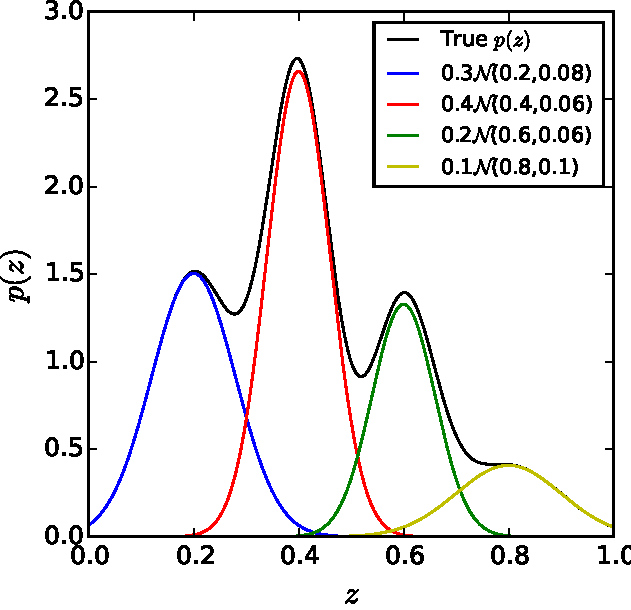
\includegraphics[width=0.5\textwidth]{figs/null/physPz.pdf}\\
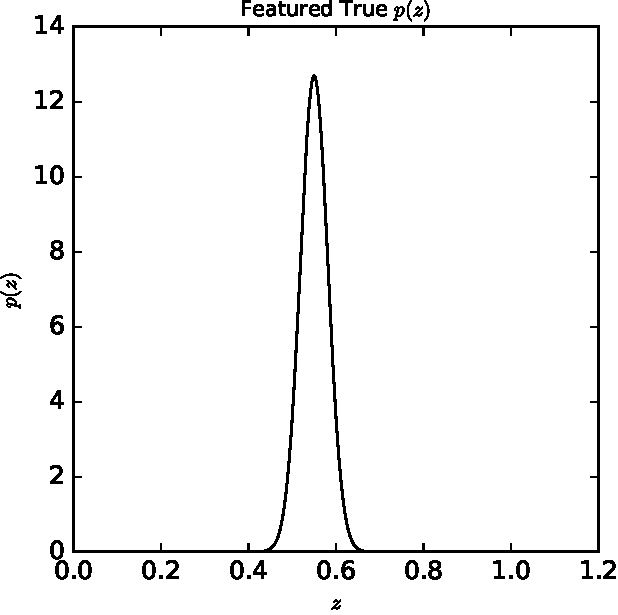
\includegraphics[width=0.5\textwidth]{figs/delt/physPz.pdf}
\caption{The physically-motivated true redshift distribution (black line) used 
in the mock data tests is chosen to have recognizable features of different 
scales so the quality of recovery can be easily determined.  The top panel 
shows a physically motivated true $N(z)$ for the fiducial test, and the bottom 
panel shows a toy model of a highly featured true $N(z)$.}
\label{fig:physpz}
\end{figure}

The catalog of $J$ photo-$z$ likelihoods $p(\vec{d}_{j}|z_{j})$ is chosen to be 
a set of Gaussian distributions, truncated to the redshift range over which 
$N(z)$ is defined, because it is the simplest extension of the standard 
redshift point estimates with reported error bars.  To obtain the standard 
deviations $\sigma_{j}\sim\mathcal{N}(g\bar{\Delta},(g\bar{\Delta})^{2})$ 
associated with each surveyed galaxy $j$, we first sample a Gaussian 
distribution with mean and standard deviation equal to $g\bar{\Delta}$ for some 
factor $g$ (by default set to unity), truncated to enforce positive standard 
deviations.  Each Gaussian is centered at an "observed" redshift 
$z'_{j}\sim\mathcal{N}(z^{*}_{j},\sigma_{j})$ separated from the true redshift 
$z^{*}_{j}$ by a Gaussian random variable 
$\epsilon_{j}\sim\mathcal{N}(0,\sigma^{2}_{j})$ selected from a distribution of 
mean of 0 and true standard deviation $\sigma_{j}$.   This prescription may be 
understood as an exposition of the generative model of 
\begin{equation}
\label{eq:genmod}
z'_{j} = z^{*}_{j}+\epsilon_{j}
\end{equation}
for the physically-motivated process originating the data, which states that 
the MLE $z'_{j}$ of the redshift is equal to the true redshift $z^{*}_{j}$ plus 
a Gaussian random variable $\epsilon_{j}$.

We must also choose the parametrization of the redshift distribution function, 
in this case $f_{\vec{\theta}}(z)=\exp[\vec{\theta}]$ (introduced in Sec. 
\ref{sec:prob}).  We next define the elements of $\vec{\theta}$ to be log 
top-hat functions where the hyperparameters $\theta_{k}$ comprising 
$\vec{\theta}$ take values equal to $\ln[\int_{z_{k-1}}^{z_{k}}\ 
f_{\vec{\theta}}(z)\ dz]$.  By default we choose a flat distribution as the 
interim prior, but others will be tested.  (Such a comparison has been executed 
before by \citet{Viironen2015}.)

To obtain the $J$ desired interim photo-$z$ posteriors $p(z_{j}|\vec{d}_{j})$ 
from the photo-$z$ likelihoods $p(\vec{d}_{j}|z_{j})$, we simply apply Bayes' 
rule as in 
\begin{equation}
\label{eq:likpost}
p(z_{j}|\vec{d}_{j}) \propto p(\vec{d}_{j}|z_{j})\ p(z_{j}|\vec{\theta}^{*}),
\end{equation}
where the prior on redshift is $p(z_{j}|\vec{\theta}^{*})$ for interim prior 
$\vec{\theta}^{*}$.  There are two unknown constants of proportionality (the 
likelihood of the data $p(\vec{d}_{j})$ and $J$) that we may normalize out 
according to 
\begin{equation}
\label{eq:norm}
p(B_{k}|\vec{d}_{j}) = \frac{\int_{z_{k-1}}^{z_{k}}\ p(\vec{d}_{j}|z_{j})\ 
\exp[\vec{\theta}^{*}]\ dz_{j}}{\int_{z_{min}}^{z_{max}}\ p(\vec{d}_{j}|z_{j})\ 
\exp[\vec{\theta}^{*}]\ dz_{j}}.
\end{equation}
A random sampling of such interim redshift posteriors are shown in Fig. 
\ref{fig:nullpzs}.  

\begin{figure}
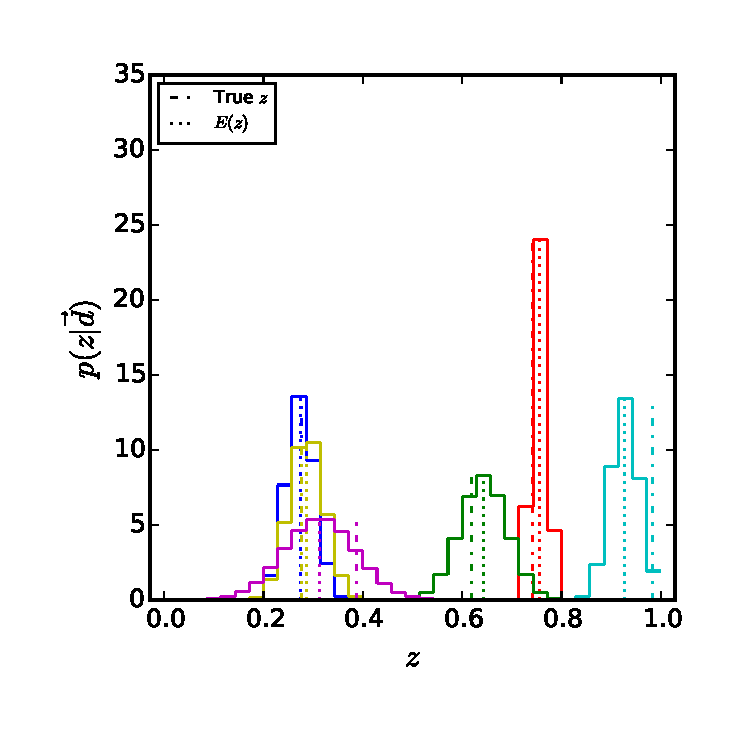
\includegraphics[width=0.5\textwidth]{figs/null/samplepzs.pdf}
\caption{Several examples of individual photo-$z$ posteriors and their MLE 
redshifts are shown in colors, along with their true redshifts.  The fiducial 
case has likelihoods comprised of a single Gaussian distribution with a known 
standard deviation centered at a shifted redshift (dotted lines) separated from 
the true redshift (dashed lines) by a Gaussian random variable with the same 
standard deviation.}
\label{fig:nullpzs}
\end{figure}

\subsubsection{Imprecise Data}
\label{sec:imprecision}

Several factors contribute to photometric redshifts' intrinsic scatter.  
Distant galaxies are dimmer compared to galaxies of identical luminosity that 
are closer, driving up photometric errors in flux-limited surveys.  The nature 
of the galaxy sample at higher redshifts also changes, meaning the generation 
of the photometric redshift posterior based on an a locally-calibrated SED 
template library or spectroscopically-confirmed training is more likely to be 
inappropriate, leading to broader features.  In general, the galaxies that 
could not have been observed spectroscopically will have different and noisier 
photo-$z$ PDFs than those that could fall into a spectroscopic training set.

Here we vary the fiducial case with noisier data to demonstrate that the 
results of the sampler and of stacking diverge for broader photo-$z$ 
likelihoods.  In these cases, $\sigma_{j}$ is drawn from a normal distribution 
as described in Sec. \ref{sec:mock} but with the factor $f=2$ ("doubly 
imprecise" compared to the fiducial case) in one case and $f=4$ ("quadruply 
imprecise" compared to the fiducial case) in another.  In both cases, 
illustrated in Fig. \ref{fig:sigspzs}, the corresponding sample interim 
photo-$z$ posteriors to those of Fig. \ref{fig:nullpzs} are broader, with MLE 
redshifts farther from the true redshift on average.

\begin{figure}
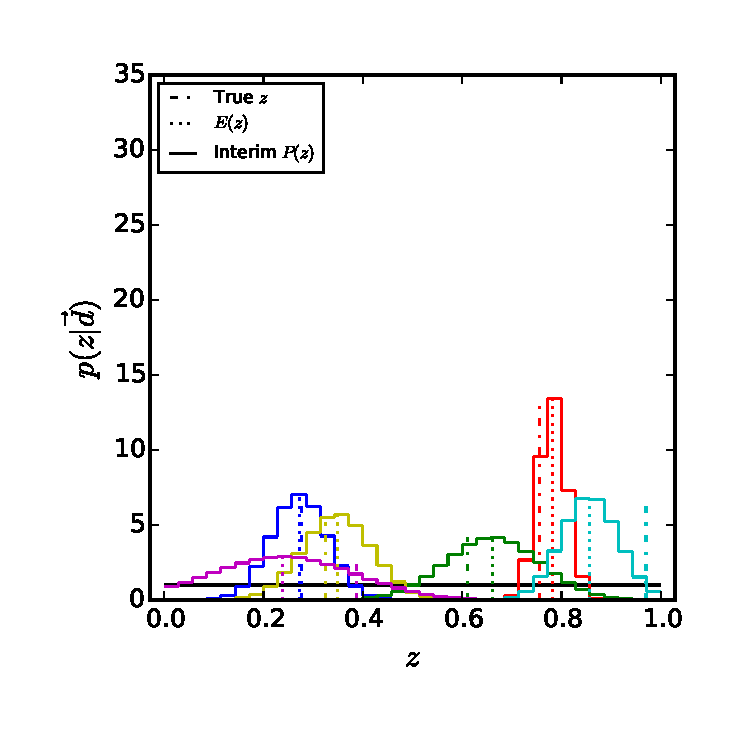
\includegraphics[width=0.5\textwidth]{figs/sig2/samplepzs.pdf}\\
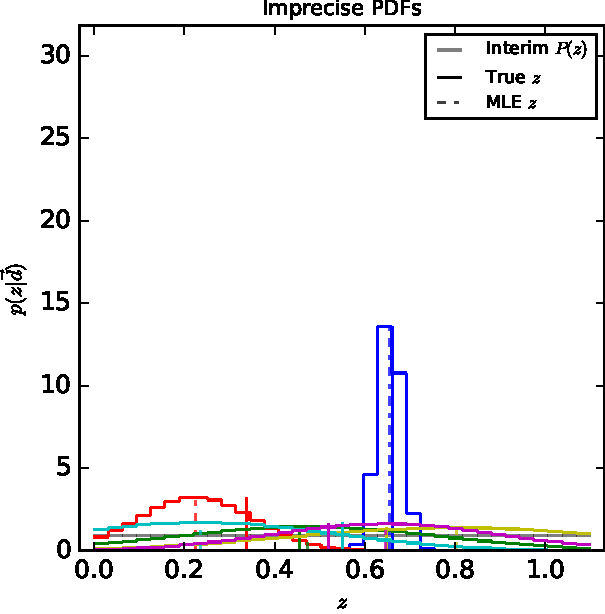
\includegraphics[width=0.5\textwidth]{figs/sig4/samplepzs.pdf}
\caption{Same as Fig \ref{fig:nullpzs}.  The doubly imprecise (top panel) and 
quadruply imprecise PDFs (bottom panel) cases have standard deviations are 
increased by a factor of 2 or 4 respectively.}
\label{fig:sigspzs}
\end{figure}

\subsubsection{Inaccurate Data}
\label{sec:inaccuracy}

In this pair of tests, we aim to simulate more realistic interim photo-$z$ 
posteriors by modifying the procedure of Sec. \ref{sec:mock} to introduce 
inaccuracy that causes catastrophic photo-$z$ errors.  Catastrophic photo-$z$ 
errors arise from a degeneracy in the space of galaxy SEDs and redshifts, 
wherein a galaxy of one SED type at one redshift has photometry 
indistinguishable from a galaxy of another SED type at another redshift.  In 
this case, the Gaussian components of the likelihood may have standard 
deviations that do not correspond to the true standard deviation used to 
generate the data, or there may be multiple components to the interim photo-$z$ 
posteriors.  Both cases will be considered here by introducing one change in 
the steps of Sec. \ref{sec:mock}.  

The first case modifies the generative model of (\ref{eq:genmod}) to have 
$\epsilon_{j}\sim\mathcal{N}(0,\sigma'^{2}_{j})$ for 
$\sigma'_{j}\sim\mathcal{N}(\bar{\Delta},\bar{\Delta}^{2})$.  This modification 
is reflected in the interim photo-$z$ posteriors, a sampling of which is shown 
in the top panel of Fig. \ref{fig:allpzs}.  In the second test case of 
inaccurate photo-$z$ posteriors, catastrophic errors are simulated by 
considering multimodal photo-$z$ likelihoods.  To achieve this goal we 
introduce another change in Sec. \ref{sec:mock}.  Here, the redshift posteriors 
are sums of Gaussians of the form of those tested in Sec. \ref{sec:null}.  Each 
galaxy is assigned a number $R_{j}$ of Gaussian elements to be summed, chosen 
randomly from $1,\dots,K$ with weights proportional to $k^{-1}$.  One 
$\sigma_{jr}$ is drawn for each $r=1,\dots,R_{j}$, and one $z'_{jr}$ is 
selected from the corresponding $\mathcal{N}(z^{*}_{j},\sigma^{2}_{jr})$.  The 
components are summed and normalized to yield the likelihood, which is then 
convolved with the interim prior to produce a true interim posterior, which is 
sampled $K$ times and renormalized to produce the final interim posterior used 
in the analysis.  Some examples of the multimodal interim photo-$z$ posteriors 
are shown in the bottom panel of Fig. \ref{fig:allpzs}.    

\begin{figure}
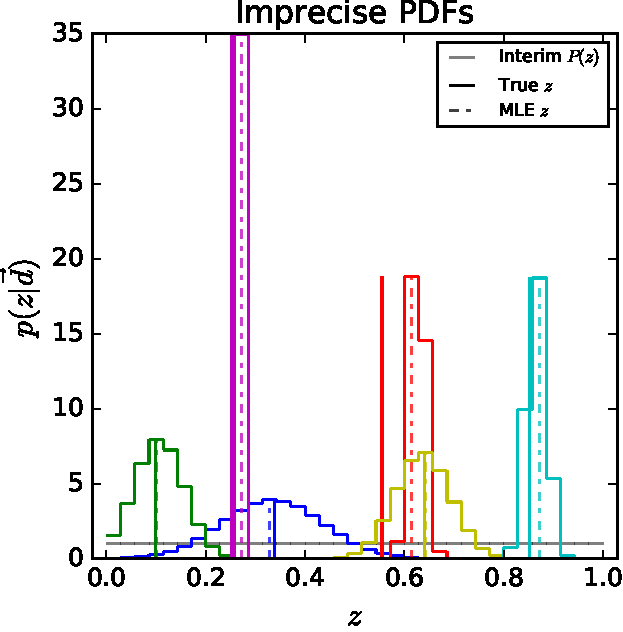
\includegraphics[width=0.5\textwidth]{figs/vars/samplepzs.pdf}\\
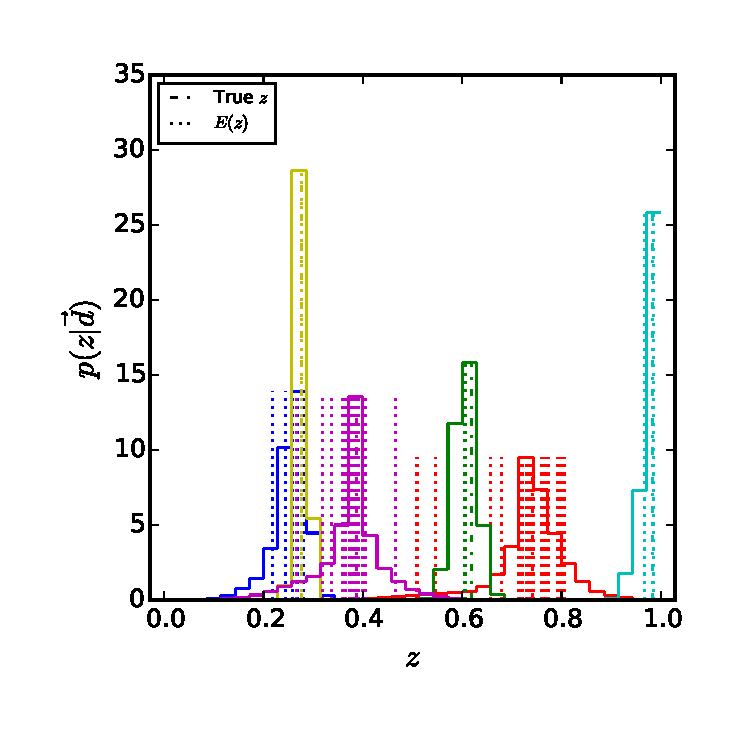
\includegraphics[width=0.5\textwidth]{figs/mult/samplepzs.pdf}
\caption{Same as Fig. \ref{fig:nullpzs}.  The imprecise PDFs case (top panel) 
differs in that the generative model for the data is violated.  The inaccurate 
PDFs case (bottom panel) shows the same quantities as the other panels but for 
multimodal and asymmetric PDFs, where the likelihood is a noisy sampling of a 
sum of Gaussians chosen as in the fiducial case.}
\label{fig:allpzs}
\end{figure}

\subsubsection{Toy Model}
\label{sec:fake-data}

We test the sampler in a case of a highly unrealistic but strongly featured 
true $N(z)$, that of the right panel of Fig. \ref{fig:physpz}.  This is done to 
show that the sampler works even in extreme and unanticipated conditions.  
Instead of sampling the physically motivated true distribution 
$p(z|\vec{\theta}')$ as in Sec \ref{sec:mock}, we assign all galaxies the same 
true redshift.  

\subsubsection{Variable Interim Prior}
\label{sec:interim}

In the following two cases we vary the interim prior used in Sec. 
\ref{sec:mock} to show that the sampler is robust to inappropriate choices of 
interim prior so long as that interim prior is known.  Typically, interim 
redshift posteriors are made with an interim prior derived from $N(z)$ in a 
previous observational study.  Since most observational studies used for this 
purpose are spectroscopically confirmed and objects for which photometric 
redshifts are relied upon make up a population that cannot be spectroscopically 
confirmed, such an interim prior is rarely appropriate.  Some efforts have been 
made to modify an observationally informed interim prior so that it is more 
representative of the data set \citep{Sheldon2012}.  However, any interim prior 
of this kind imparts information into the interim redshift posteriors.  
Ideally, an uninformative interim prior would be used, although it may be 
complicated to compute from the covariances of the raw data.  In this test, we 
consider two obviously inappropriate interim priors and compare the result to 
that of the flat interim prior used in previous tests according to Sec. 
\ref{sec:mock}.

In some cases, the interim prior is chosen to be the final product of a 
previously conducted spectroscopic redshift survey.  Because low-redshift 
galaxies are more likely to be bright enough to be observed by such a survey, 
$N(z)$ determined from that sample may be heavily biased to low redshift 
galaxies.  By contrast, the galaxies that were unobserved in such a survey are 
more likely be dimmer, making them more likely to be at higher redshifts.  
Since the interim prior is not compatible with our beliefs about the true 
redshift distribution, the resulting interim redshift posteriors will be 
inappropriate.  In this test, we choose an interim prior with most of its 
weight at low redshifts and observe its influence on the recovery of the true 
$N(z)$ by different methods.  

Another potential method for selecting an interim prior with support over the 
entire redshift range expected of the photometric survey is to sum two or more 
$N(z)$ distributions obtained from reliable photometric surveys in the past.  
This is just as problematic as using a biased spectroscopically derived $N(z)$ 
as the interim prior because the sum of redshift distributions for two or more 
surveys does not reflect our beliefs about the true distribution for a single 
survey even though it provides support over the same redshift range.  To 
simulate this case, we choose an interim prior with more weight at high and low 
redshifts than for mid-range redshifts.  

%\clearpage
\subsubsection{BOSS Data}
\label{sec:data}

We also test this method on subsets of the published interim photo-$z$ 
posteriors of SDSS III DR 10.  A sampling of the provided interim photo-$z$ 
posteriors of dimension $K=35$ for $z_{min}=0.3$ and $z_{max}=1.4$ is shown in 
the lower panels of Fig. \ref{fig:datapzs}.  The interim prior used for this 
set of interim redshift posteriors is the reweighted estimator of $N(z)$ of 
\citet{Sheldon2012}.

\begin{figure}
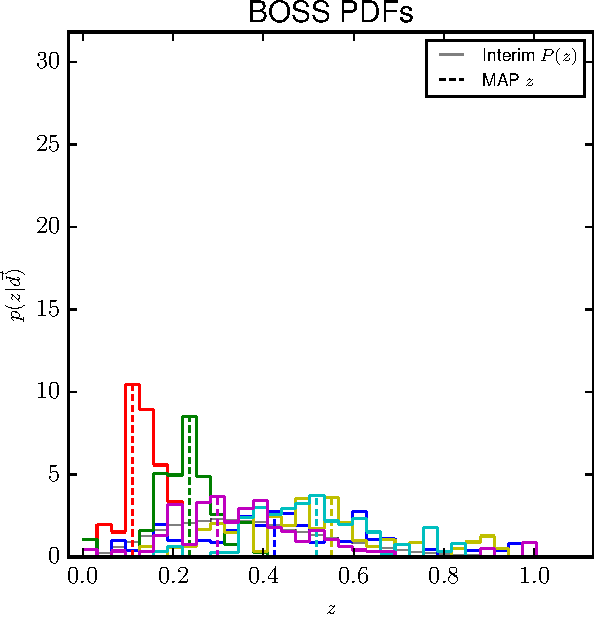
\includegraphics[width=0.5\textwidth]{figs/boss/samplepzs.pdf}\\
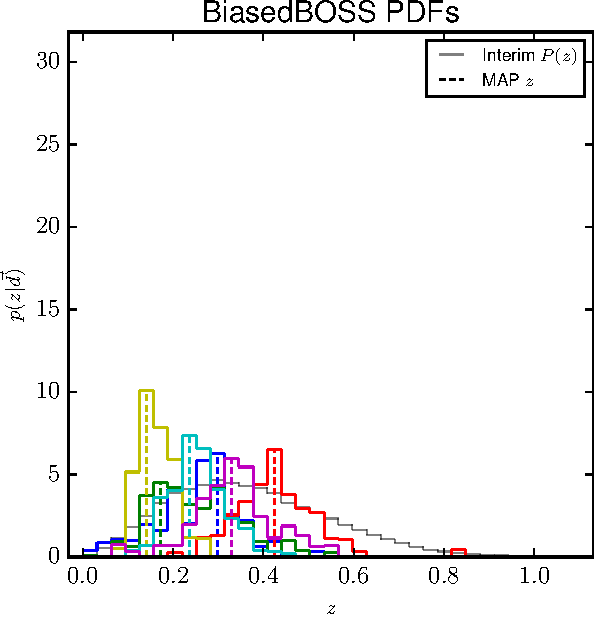
\includegraphics[width=0.5\textwidth]{figs/bias/samplepzs.pdf}
\caption{Here is shown the same information as in Fig. \ref{fig:nullpzs} for 
real data.  A pseudo-random sampling of BOSS DR 10 photo-$z$ posteriors 
produced by \citet{Sheldon2012} (top panel) are clearly much noisier than those 
of the fiducial case.  A random sampling of the brightest half of the 
pseudo-random BOSS DR10 sample (bottom panel) corresponds to much cleaner 
photo-$z$ PDFs.}
\label{fig:datapzs}
\end{figure}

In addition to simulated tests, we also apply this method to a samples of the 
data described in Sec. \ref{sec:data}.  The interim prior is taken from 
\citet{Sheldon2012}.  In these cases the true $N(z)$ is not known, but the 
fully probabilistic method presented here may still be compared to what is 
obtained by alternative approaches.

A pseudo-random sampling of the full BOSS dataset is first examined to 
approximate the behavior of an average galaxy survey.  Samples of photo-$z$ 
interim posteriors are shown in the left panel of Fig. \ref{fig:datapzs}.  

%\clearpage
\subsection{Implementation Details}
\label{sec:mcmc}

The testing procedure is implemented in \texttt{Python} and is made public as 
Cosmological Hierarchical Inference with Probabilistic Photometric Redshifts 
(CHIPPR).  The code takes as input a \texttt{csv} file containing the basis for 
the binning of redshift space, a specification of the interim prior 
$\vec{\theta}^{*}$, and a catalog of $J$ interim photo-$z$ log-posteriors 
$\{\ln[p(B_{j}|\vec{d}_{j},\vec{\theta}^{*})]\}_{J}$.

The \texttt{emcee} \citep{Foreman-Mackey2013} implementation of ensemble 
sampling is applied to sample the full log-posterior of (\ref{eq:final}).   For 
each of some $W$ walkers at each iteration $i$, a proposal distribution 
$\vec{\theta}^{i}$ generated from the hyperprior distribution and evaluated for 
acceptance to or rejection from the desired log-posterior distribution.  Two 
threshold conditions are defined, one designating all previous samples to be 
ignored as as products of a "burn-in" phase and another indicating when a 
sufficient number of "post-burn" samples have been accepted.  In this case, the 
first threshold (described in Sec. \ref{sec:acorr}) is defined in terms of 
sub-runs of $I_{0}=10^{3}$ accepted samples, and the second is defined as an 
accumulation of $I_{tot}=10^{4}$ samples.

The sampler is initialized with $M=100$ walkers each with a value chosen from a 
Gaussian distribution of identity covariance around a sample from the 
hyperprior distribution.  An example of such samples from the prior are shown 
in Fig. \ref{fig:prior}.

\begin{figure}
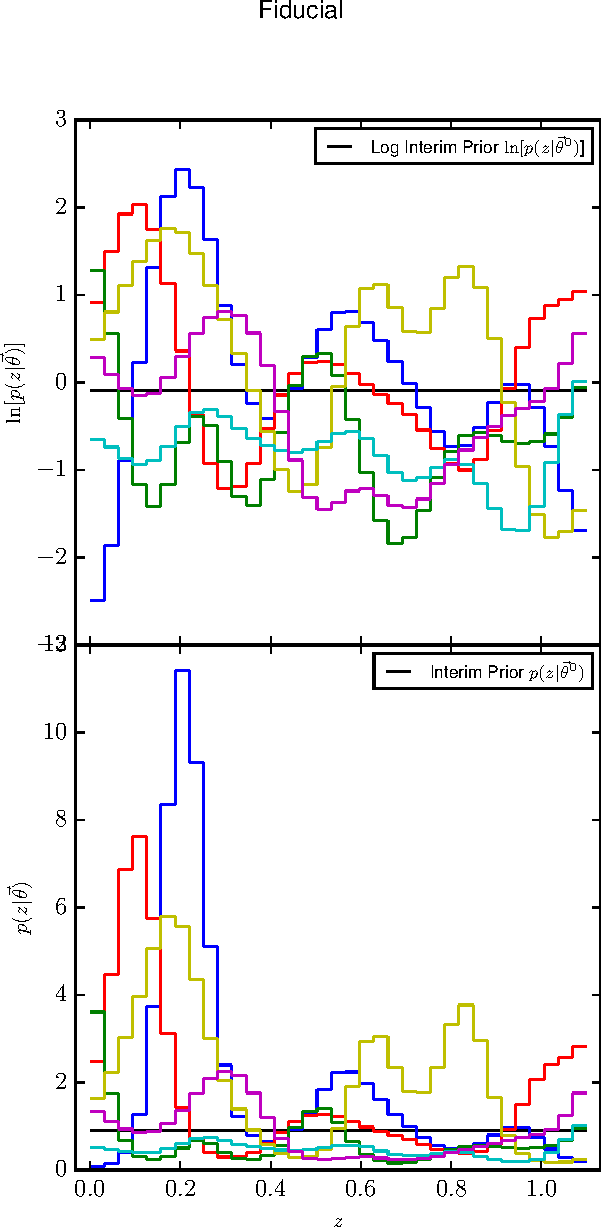
\includegraphics[width=0.5\textwidth]{figs/null/priorsamps.pdf}
\caption{This figure shows samples (colored lines) of $p(z|\vec{\theta})$ where 
each $\vec{\theta}$ is drawn from the hyperprior distribution $p(\vec{\theta})$ 
defined in Sec. \ref{sec:exp} with \ref{eq:priorcov}.}
\label{fig:prior}
\end{figure}

The input/output format chosen for this work is \texttt{HDF5} because of its 
efficiency for large amounts of data.  The resulting output is a set of $I$ 
ordered \texttt{hickle} files enumerated by $\rho$ containing the state 
information after each sub-run.  The state information includes 
$\frac{I_{0}}{s}$ actual samples $\vec{\theta}_{i}$ for a pre-specified chain 
thinning factor $s$ and their full posterior probabilities 
$p(\vec{\theta}_{i}|\{\vec{d}_{j}\})$ as well as the autocorrelation times and 
acceptance fractions calculated for each element of $\vec{\theta}$ over the 
entire sub-run.  

%\clearpage
\subsubsection{Convergence Criteria}
\label{sec:acorr}

In addition to qualitative visual inspection of the chains, two quantities that 
probe the convergence of the sampler are used in this study, the 
autocorrelation time and the Gelman-Rubin convergence criterion.  Fig. 
\ref{fig:chains} shows the evolution of the values of one parameter of one 
walker over the course of all iterations of the sampler.

\begin{figure}
%\includegraphics[width=0.5\textwidth]{figs/null/chain0.pdf}
\caption{This figure shows the evolution of one walker's parameter values for 
one element of the parameter vector $\vec{\theta}$ as a function of iteration 
number, demonstrating the completion of the burn-in phase.}
\label{fig:chains}
\end{figure}

The autocorrelation time is effectively a measure of the efficiency of the 
method and can be described as the expected number of iterations necessary to 
accept a new sample independent of the current accepted sample.  A sampler that 
converges faster will have a smaller autocorrelation time, and smaller 
autocorrelation times are preferable because it means fewer iterations are 
wasted on non-independent samples when independent samples are desired.  See 
\citet{Foreman-Mackey2013} for a more complete exploration of the 
autocorrelation time.  In all tests discussed here, autocorrelation times 
across walkers and parameters were approximately 20, meaning two samples 20 or 
more iterations apart were independent, a satisfactory level of efficiency.  
Low autocorrelation times are a necessary but not always sufficient convergence 
condition, as the autocorrelation times calculated for tests in this paper were 
constant across all sub-runs, even those that were obviously burning in.  

The Gelman-Rubin statistic
\begin{equation}
\label{eq:gr}
R_{k} = \sqrt{\frac{(1-\frac{2}{I_{0}})w_{k}+\frac{2}{I_{0}}b_{k}}{w_{k}}},
\end{equation}
a weighted sum of the mean $w_{k}$ of the variances within individual walkers' 
chains and the variance $b_{k}$ between chains of different walkers $m$, is 
calculated over each sub-run $i$ to determine the duration of the burn-in 
period.  Convergence is achieved when the statistic approaches unity.  

%\clearpage
\subsection{Diagnostics}
\label{sec:diag}

The results of the computation described in Sec. \ref{sec:mcmc} are evaluated 
for accuracy on the basis of some quantitative measures.  Beyond visual 
inspection of samples, we calculate summary statistics to quantitatively 
compare different estimators' precision and accuracy.  Since MCMC samples of 
hyperparameters are Gaussian distributions, we can quantify the breadth of the 
distribution for each hyperparameter using the standard deviation regardless of 
whether the true values are known.  

In simulated cases where the true parameter values are known, we calculate the 
Kullback-Leibler divergence (KLD), given in 
\begin{equation}
\label{eq:kl}
KL_{\dagger,'} = \sum_{k=1}^{K}\ \exp[\theta_{k}^{\dagger}]\ 
\ln\left[\frac{\theta_{k}^{\dagger}}{\theta_{k}^{'}}\right]\ \Delta_{k},
\end{equation}
which measures a distance between parameter values $\vec{\theta}^{\dagger}$ and 
$\vec{\theta}^{'}$ that is invariant under changes of variables.  We note that 
$KL_{\dagger,'}\neq KL_{',\dagger}$, so both must be calculated, and the 
minimum of the two is reported in this study.  In simulated tests, one of 
$\vec{\theta}^{\dagger}$ and $\vec{\theta}^{'}$ is the true value and the other 
is the value produced by one of the methods in question.  

%\clearpage
\section{Validation Tests}
\label{sec:valid}

\textbf{This is the section that's weakest, and, I am aware, also the most 
important.  I could use some concrete recommendations of how to change it to be 
publishable.}

Here we present the results of the informative tests of Sec. \ref{sec:exp}, 
summarized in Tab. \ref{tab:key}.  

%\clearpage
\subsection{Fiducial Case}
\label{sec:null}

For the fiducial experiment, we precisely follow the procedures outlined in 
Sec. \ref{sec:mock} and Sec. \ref{sec:mcmc}.  Recall that Fig. 
\ref{fig:nullpzs} shows the interim photo-$z$ posteriors used in this test 
case.  Fig. \ref{fig:null-samp} shows some random sample values, the true value 
of $N(z)$.  Fig. \ref{fig:null-comp} compares the mean of the sample values to 
alternative estimators as well as the truth.

\begin{figure}
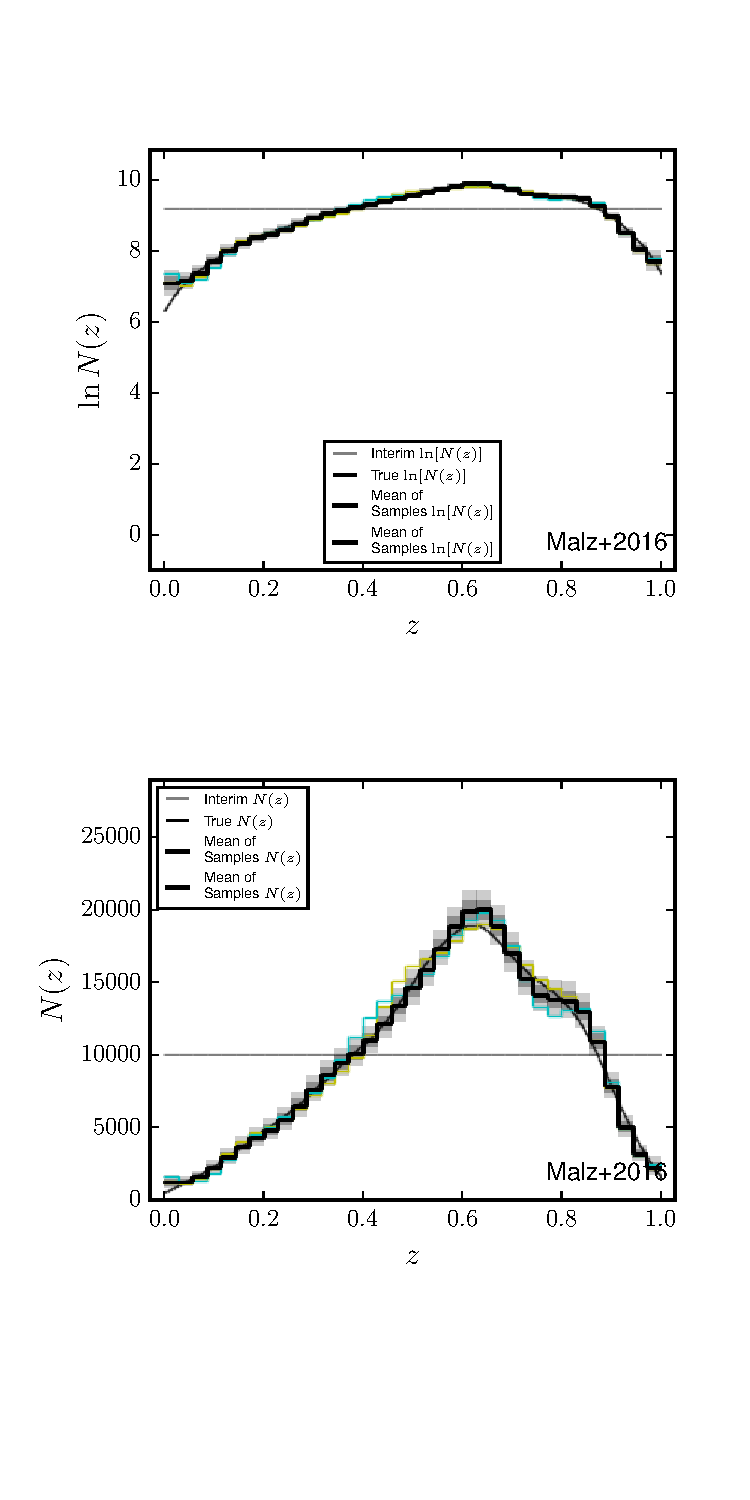
\includegraphics[width=0.5\textwidth]{figs/null/samps.pdf}
\caption{This test was conducted with a flat interim prior (gray line) and 
produced a mean of samples (thick, black line) that accurately reproduces the 
truth.  It can be seen that the samples (colored lines) are an excellent 
estimator of the true $N(z)$ (thin, black line) with the true values falling 
within the error bars ($1\sigma$ in dark gray, $2\sigma$ in light gray).}
\label{fig:null-samp}
\end{figure}

\begin{figure}
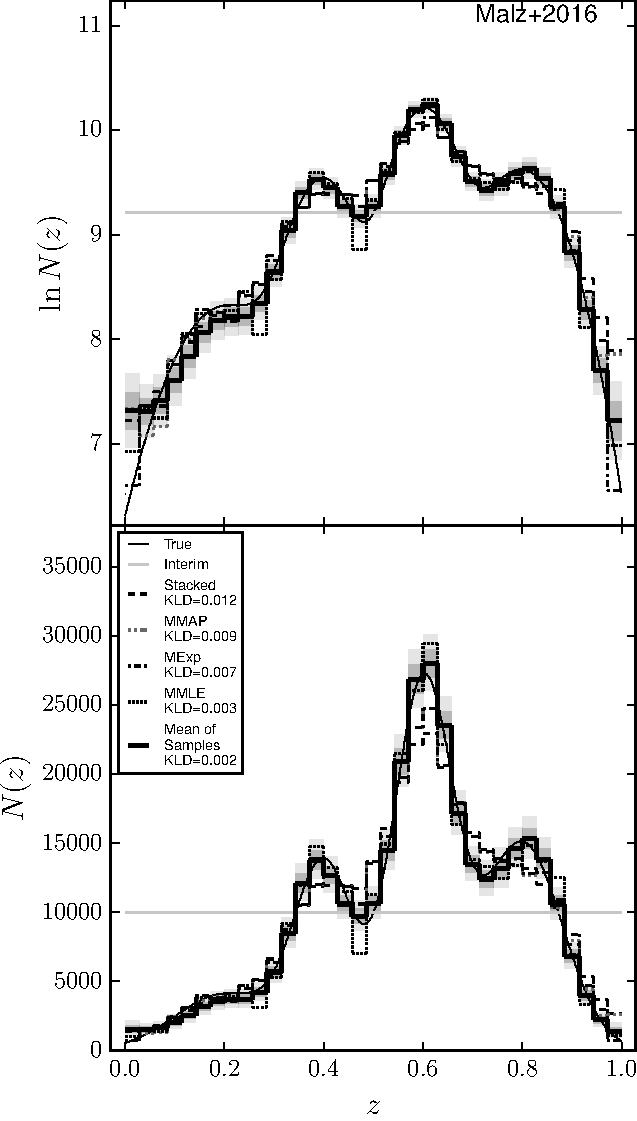
\includegraphics[width=0.5\textwidth]{figs/null/comps.pdf}
\caption{The mean of the samples (thick, solid line; KLD $0.002$) and 
marginalized MLE (thick, dotted line; KLD $0.003$) are the best estimators of 
the true distribution (thin, black line); stacking (thick, dashed line; KLD 
$0.012$) overestimates $N(z)$ at the tails and underestimates $N(z)$ at the 
peaks.  The two point estimators considered here, marginalized MAP (thin, 
dashed line; KLD $0.009$) and marginalized expected value (thin, dotted line; 
KLD $0.007$) fall between these two extremes.}
\label{fig:null-comp}
\end{figure}

In the fiducial case, hierarchical inference preserves features in the redshift 
distribution function, whereas stacking tends to smear them out.  The 
difference between stacking and the mean of the samples is more evident in 
cases of noisier data, discussed in Sec. \ref{sec:noisy}.

%\clearpage
\subsection{Imprecise interim photo-$z$ posteriors}
\label{sec:noisy}

The sampler was run on the two, noisier datasets described in Sec. 
\ref{sec:noisy-data} with broader likelihoods and produced broader error bars 
on the mean of the samples, with little effect on the value of the mean of the 
samples.  Fig. \ref{fig:sig4-comp} shows this result for the $f=4$ case.  The 
alternative methods are more strongly affected by the broadened likelihoods; as 
the standard deviation of the photo-$z$ likelihood functions increases, the 
stacked result becomes so broad as to erase all features from the estimate of 
$N(z)$, while the marginalized MLE enhances peaks and troughs to bias the 
estimate.

%\begin{figure}
%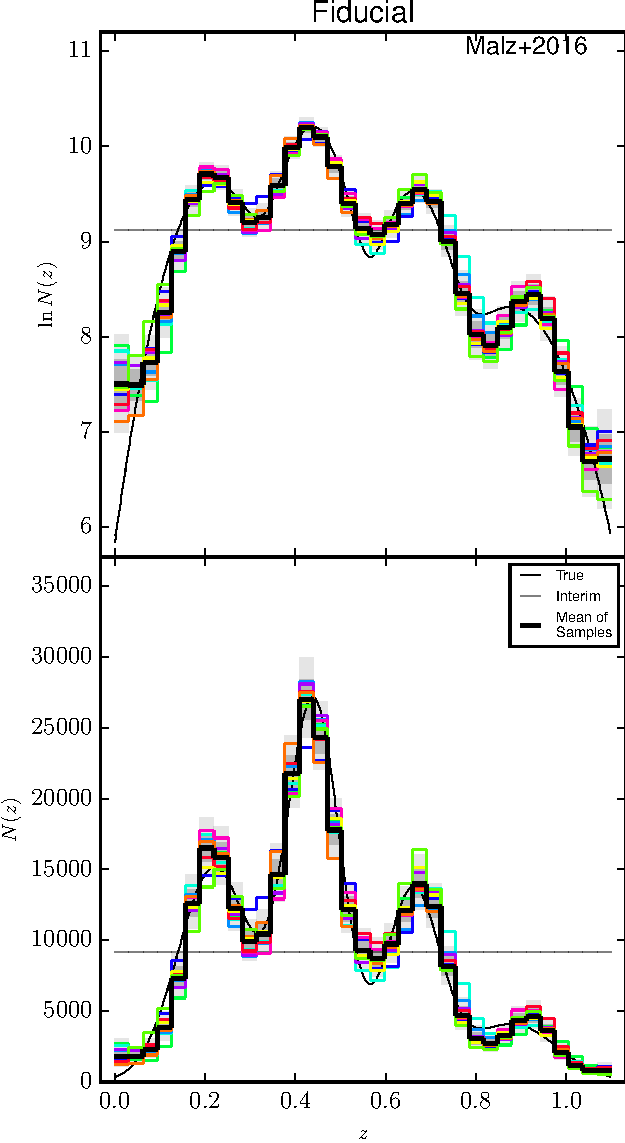
\includegraphics[width=0.5\textwidth]{figs/sig2/samps.pdf}
%\caption{The mean of sampled values (thick, black line) is quite comparable to 
%that of the original fiducial case even though the data is twice as noisy.  How
%ever, the error bars ($1\sigma$ in dark gray, $2\sigma$ in light gray) are some
%what larger.}
%\label{fig:sig2-samp}
%\end{figure}
%
%\begin{figure}
%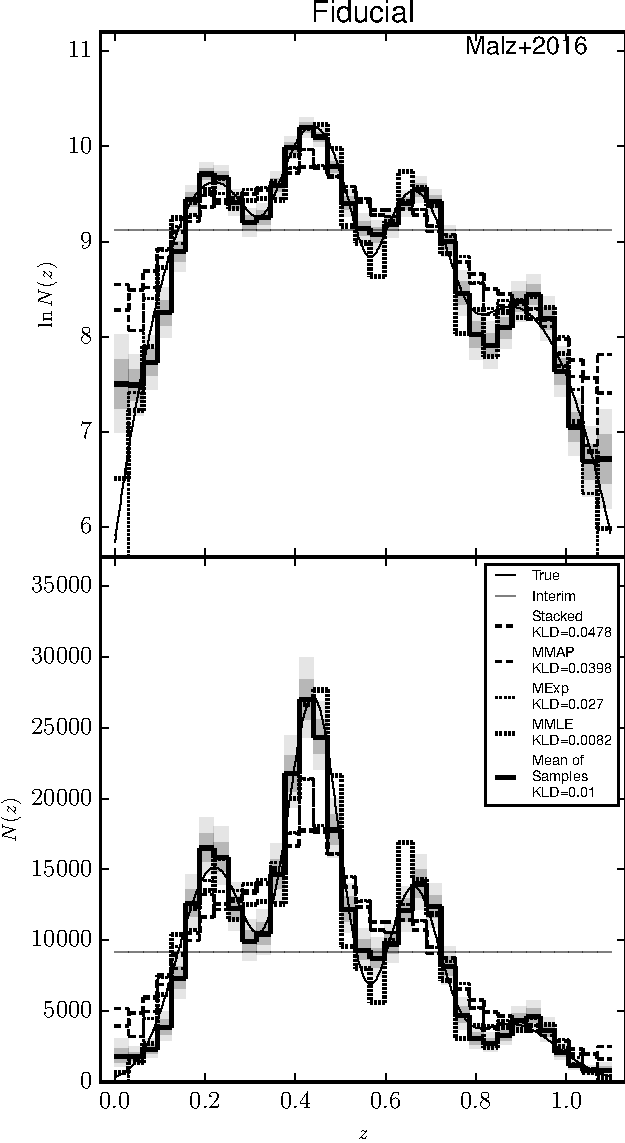
\includegraphics[width=0.5\textwidth]{figs/sig2/comps.pdf}
%\caption{The mean of sampled values (thick, black line) is prone to overestimat
%ing the peak values and underestimating the trough values relative to the true 
%$N(z)$ (thin, black line).  The result of stacking (dotted line), on the other 
%hand, underestimates the peak values, overestimates the trough values, and incr
%eases the weight of the tails, leading to a greater KLD than for the sampler.  
%The marginalized MLE (dashed line) performs well, but is more prone to the bias
%es that affect the sampler, so has a larger KLD than the sampler as well.}
%\label{fig:sig2-comp}
%\end{figure}
%
%\begin{figure}
%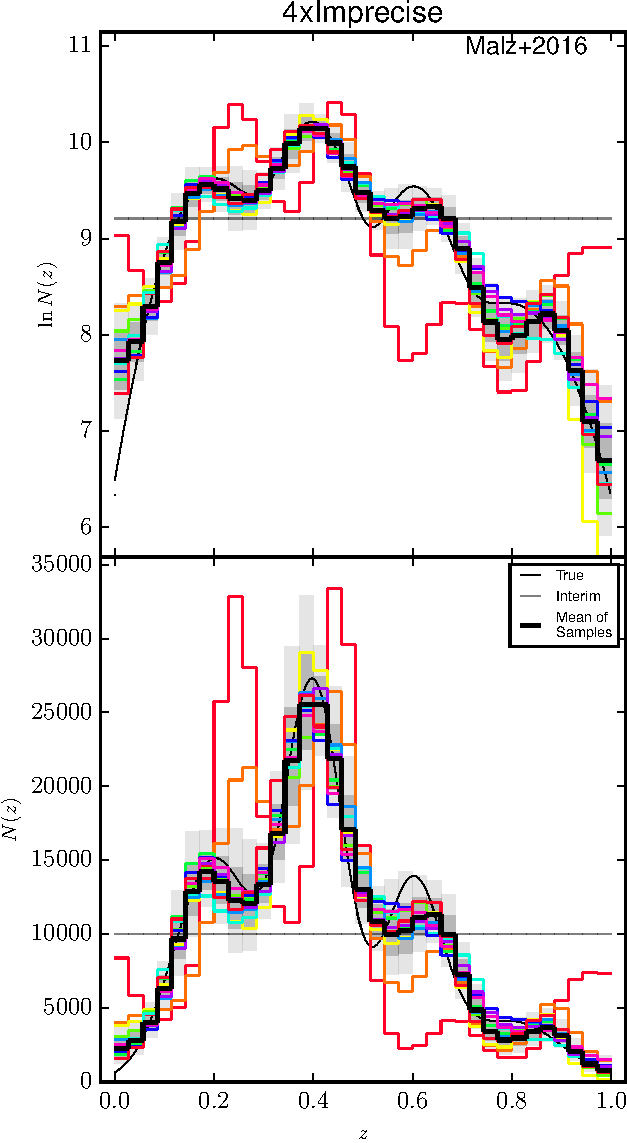
\includegraphics[width=0.5\textwidth]{figs/sig4/samps.pdf}
%\caption{Compared to Fig. \ref{fig:null-samp}, the greatest difference between 
%the original fiducial case and the quadruply noisy case is the size of the erro
%r bars ($1\sigma$ in dark gray, $2\sigma$ in light gray) about the true $N(z)$ 
%(thin, black line), as exemplified by the plotted random samples (colored lines
%) that scatter further from the mean of the sampled values (thick, black line).
%}
%\label{fig:sig4-samp}
%\end{figure}

\begin{figure}
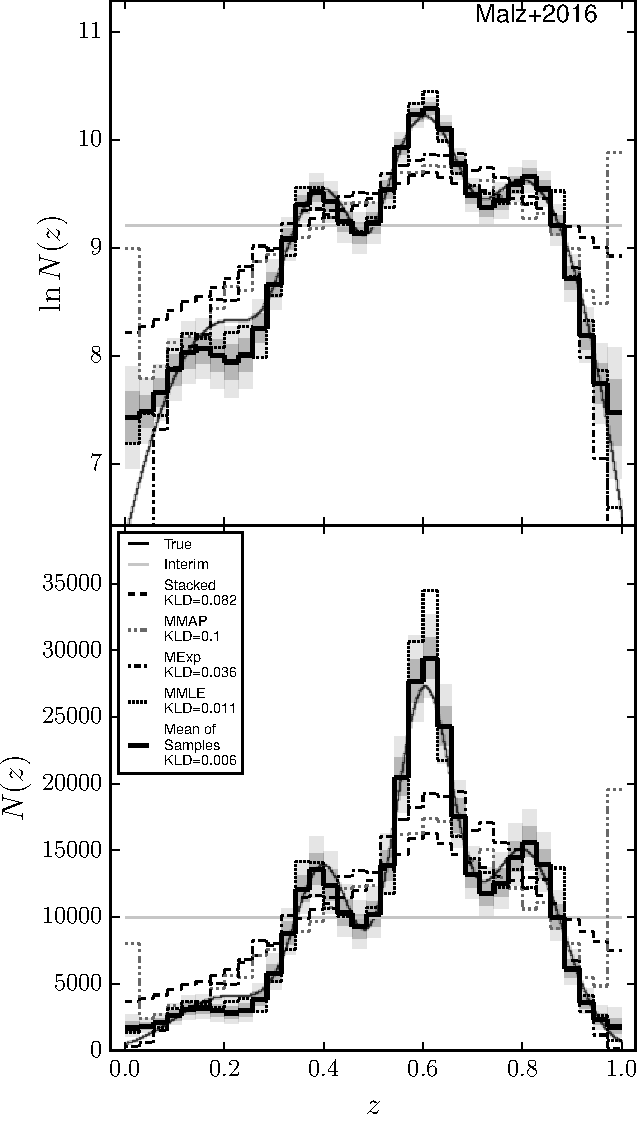
\includegraphics[width=0.5\textwidth]{figs/sig4/comps.pdf}
\caption{Here it is most obvious that the alternative methods erase features in 
estimating the true $N(z)$ (thin, black line).  The marginalized MAP (thin, 
dashed line; KLD $0.1$) is heavily biased by the systematics of the rigid 
binning but otherwise performs similarly to stacking (thick, dashed line; KLD 
$0.082$) and the marginalized expected value (thin, dotted line; KLD $0.036$), 
smoothing the features of the distribution.  The mean of sampled values (thick, 
solid line; KLD $0.006$) and marginalized MLE (thick, dotted line; KLD $0.011$) 
exhibit some bias at the peaks of the distribution but overall perform far 
better than the alternatives.}
\label{fig:sig4-comp}
\end{figure}

From these two test cases, it can be seen that the mean of the sampled 
hyperparameter values is a robust estimator of the true $N(z)$, regardless of 
the imprecision of the data.  The error bars accurately reflect our beliefs 
about the uncertainty of this estimator.  Stacking and the point estimators 
fail to recover the distinctive features of the true $N(z)$.

%\clearpage
\subsection{Inaccurate interim photo-$z$ posteriors}
\label{sec:multi}

The mean of the sampled hyperparameter values is compared to the results of 
stacking and other alternatives in Fig. \ref{fig:noisy-comp}.  It can be seen 
that inaccurate interim photo-$z$ posteriors are best handled by the sampler, 
whose KLD is lower than that of stacking and marginalized likelihood 
maximization.

%\begin{figure}
%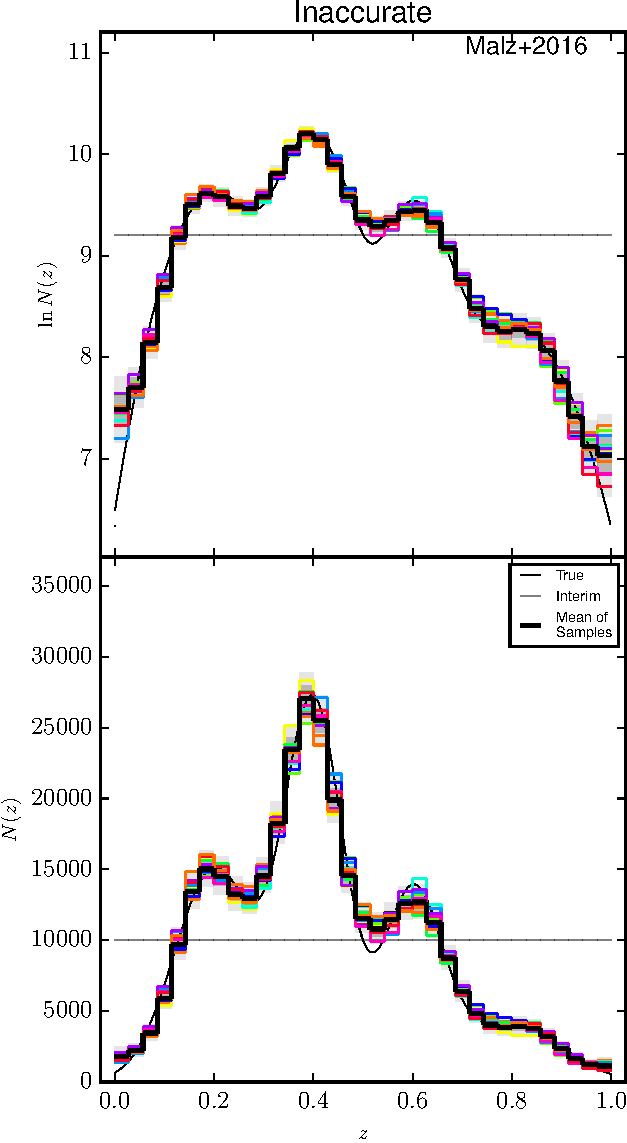
\includegraphics[width=0.5\textwidth]{figs/vars/samps.pdf}
%\caption{The mean of the sampled values (thick, black line) accurately reproduc
%es the true $N(z)$ distribution (thin, black line) such that the true values al
%ways fall within the error bars ($1\sigma$ in dark gray, $2\sigma$ in light gra
%y).  Some samples (colored lines) are shown as well.}
%\label{fig:noisy-samp}
%\end{figure}

\begin{figure}
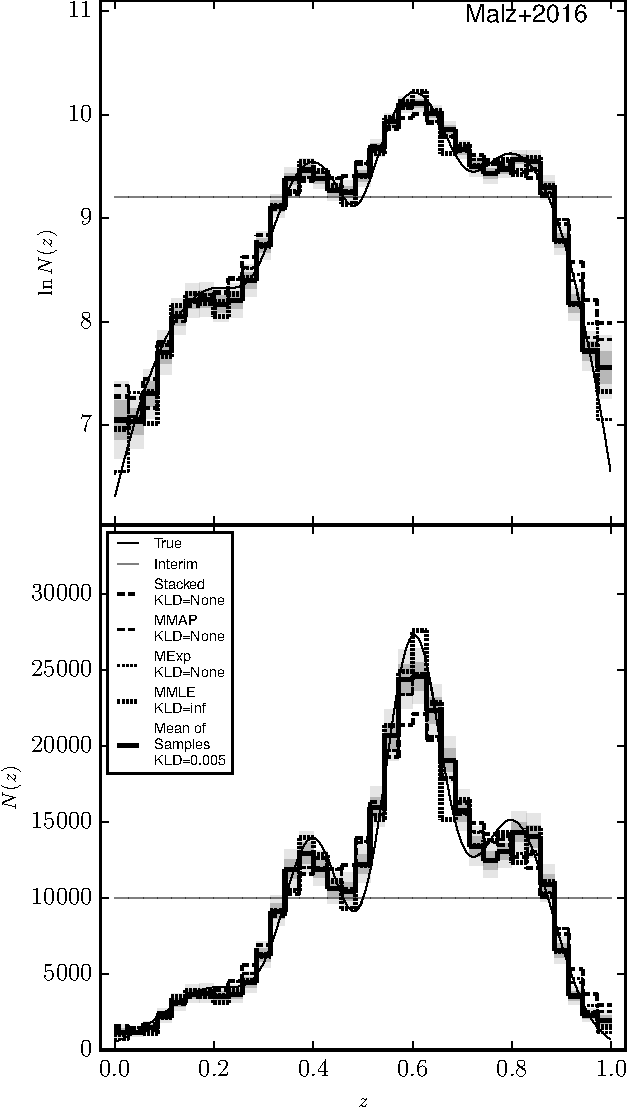
\includegraphics[width=0.5\textwidth]{figs/vars/comps.pdf}
\caption{The marginalized MLE (thick, dotted line; KLD $0.004$) is in this case 
the best estimator of the true $N(z)$.  The mean of the samples (thick, solid 
line; KLD $0.006$) shows some bias at the peaks and troughs of the 
distribution, but not as much as stacking (thick, dashed line; KLD $0.016$).  
The marginalized MAP (thin, dashed line; KLD $0.009$) and marginalized expected 
value (thin, dotted line; KLD $0.007$) have intermediate accuracy, with the 
same bias at the peaks and troughs of the distribution.}
\label{fig:noisy-comp}
\end{figure}

Fig. \ref{fig:multi-comp} shows a comparison to alternative methods.  It can be 
seen that the lessened quality of the data does impact the accuracy of the mean 
of the posterior samples as an estimator of the truth, exaggerating the signal 
at the peaks and troughs.  However, the alternatives do worse as measured by 
the KLD, with stacking smoothing the peaks and troughs.

%\begin{figure}
%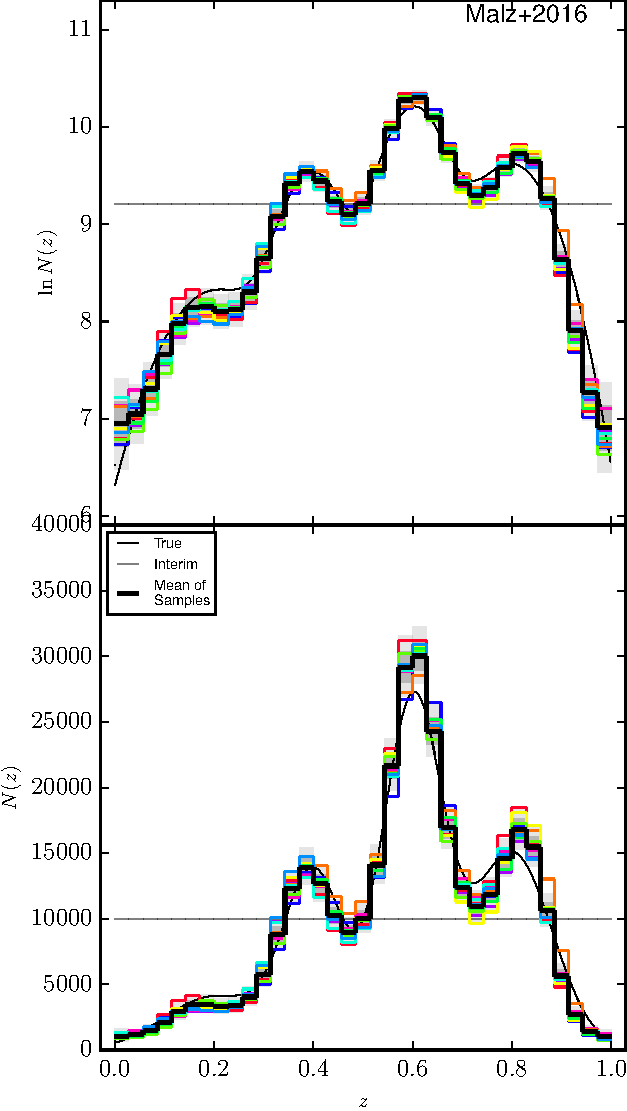
\includegraphics[width=0.5\textwidth]{figs/mult/samps.pdf}
%\caption{The mean of the sampled values (thick, black line) appears to do a rel
%atively poor job of recovering the true $N(z)$ (thin, black line), enhancing pe
%aks and troughs compared to the true distribution and underestimating the proba
%bility density in the tails.  The samples (colored lines) are quite close to th
%e mean with error bars ($1\sigma$ in dark gray, $2\sigma$ in light gray) tight 
%enough to exclude the true value.}
%\label{fig:multi-samp}
%\end{figure}

\begin{figure}
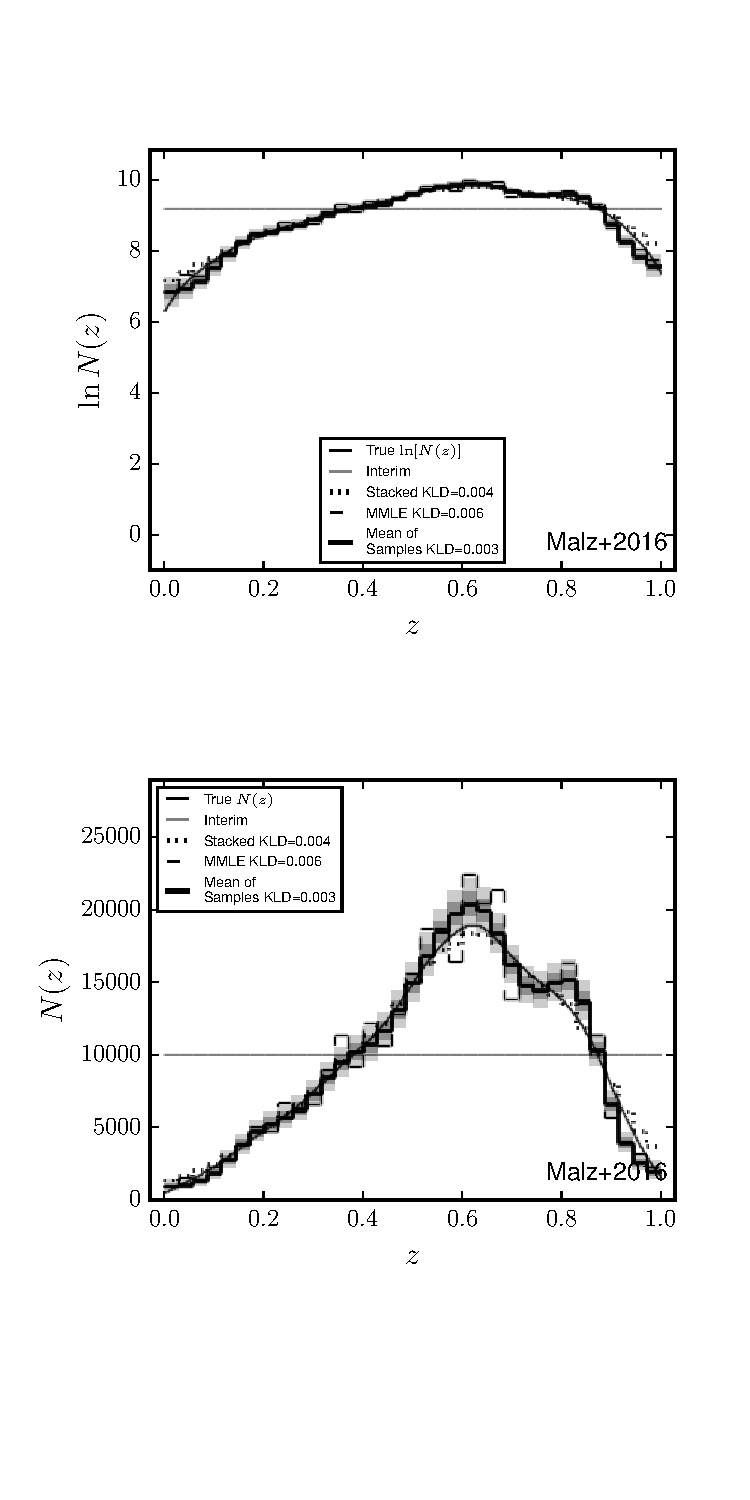
\includegraphics[width=0.5\textwidth]{figs/mult/comps.pdf}
\caption{\textbf{The point estimators are doing well because I'm not straying 
far enough from the generative model.  I will note that the MMLE has trouble 
with these kinds of distributions.}}
\label{fig:multi-comp}
\end{figure}

The performance of the mean of the samples as an estimator in these two test 
cases is weaker than in test cases that do not vary the generative model.  It 
can thus be concluded that it is essential for the success of this approach 
that the form of the likelihood passed to MCMC accurately reflect the way the 
photo-$z$ posteriors were produced.  In cases where we are uncertain as to the 
accuracy of the generative model for the photo-$z$ posteriors, it is 
recommended to use the marginalized MLE.

%\clearpage
\subsection{Toy Model $N(z)$}
\label{sec:fake}

Fig. \ref{fig:toy-comp} compares the mean of the posterior samples to the 
results of stacking and marginalized likelihood maximization.    

%\begin{figure}
%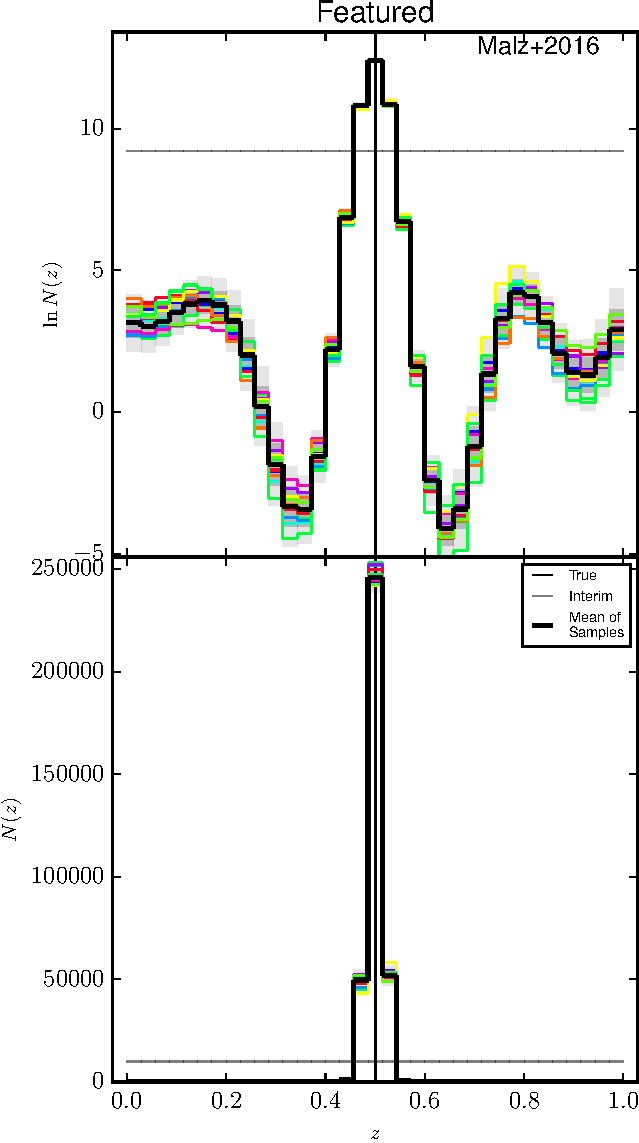
\includegraphics[width=0.5\textwidth]{figs/delt/samps.pdf}
%\caption{}
%\label{fig:toy-samp}
%\end{figure}

\begin{figure}
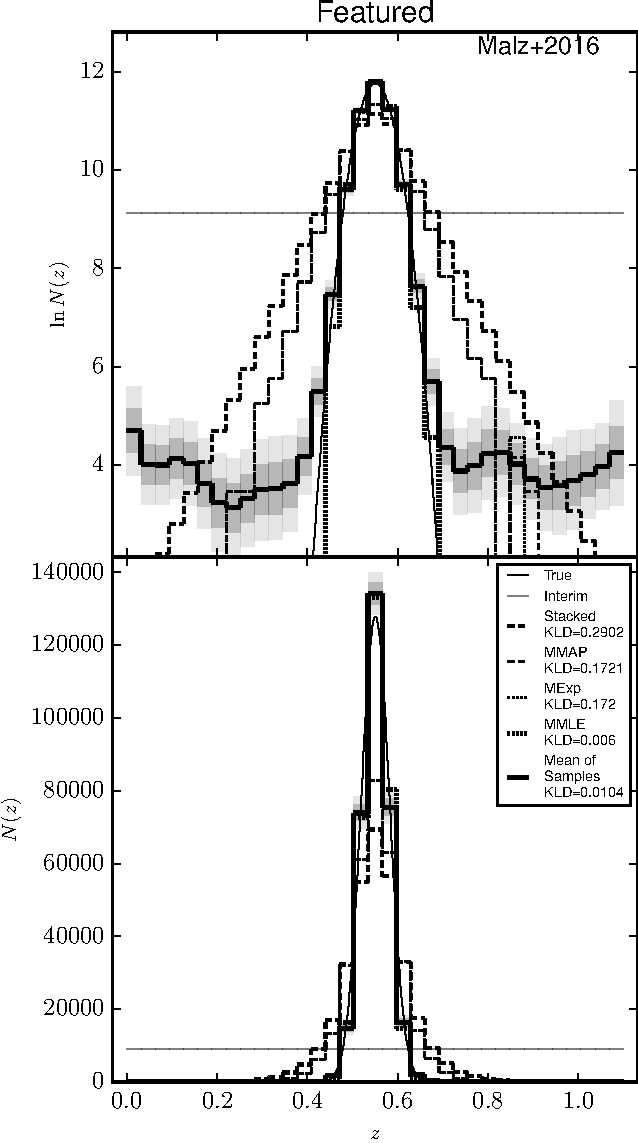
\includegraphics[width=0.5\textwidth]{figs/delt/comps.pdf}
\caption{In this case, the marginalized MLE (thick, dotted line; KLD $<0.001$) 
recovers the true $N(z)$ (thin, solid line) to greater than 0.1\% precision.  
The mean of the samples (thick, solid line; KLD $0.352$) performs almost as 
well, with some low amplitude residuals due to the form of the prior.  The 
point estimators (marginalized MAP as a thin, dashed line and marginalized 
expected value as a thin, dotted line), which share KLD $0.89$, broaden the 
distribution more than the mean of the samples but not quite as much as 
stacking (thick, dashed line; KLD $1.123$).}
\label{fig:toy-comp}
\end{figure}

It can be seen that the marginalized MLE is best at recovering the true 
distribution of a delta function due to the nature of the optimizer, which 
considers each component of the hyperparameter vector to be independent of all 
others.  Other estimators predict a broader distribution than the truth, with 
stacking broadening it the most and the mean of the samples broadening it the 
least.  Though the sampler does not consider components of the hyperparameter 
vector to be independent, it is flexible enough to provide good constraints on 
the true $N(z)$.  In cases where we expect an extremely strongly featured 
$N(z)$, such as one might find in an area with a small number of galaxy 
clusters, the marginalized MLE is the recommended estimator; if for numerical 
reasons optimization is not possible, the mean of MCMC samples is recommended.

%\clearpage
\subsection{Variable Interim Prior}
\label{sec:interim}

A comparison of the sampler to other approaches is shown in Fig. 
\ref{fig:intu-comp}.  The methods that account for the nontrivial interim prior 
(the marginalized MLE and the sampler) yield substantially less biased results 
than the methods that do not (stacking and the point estimators, the 
marginalized MAP and marginalized expected value).

%\begin{figure}
%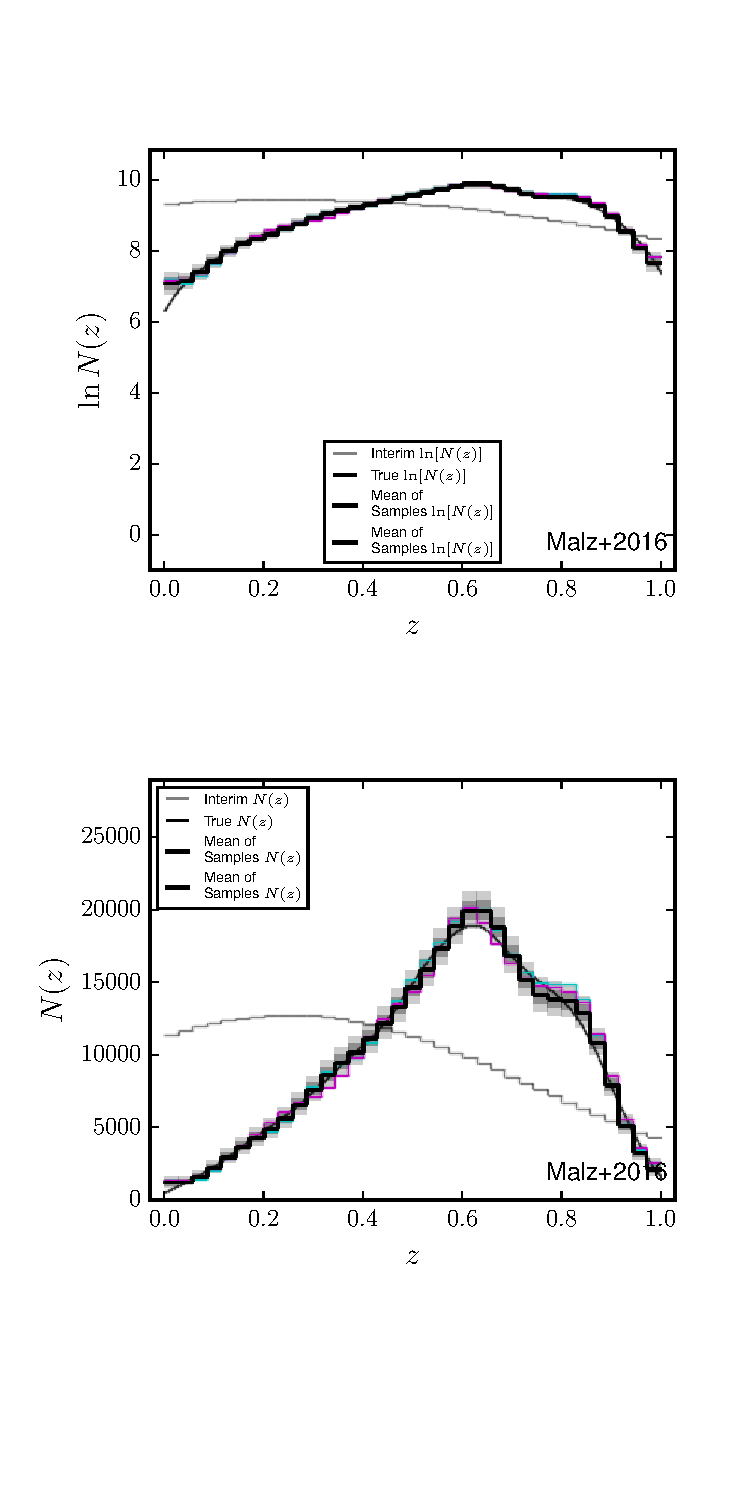
\includegraphics[width=0.5\textwidth]{figs/uint/samps.pdf}
%\caption{The mean (thick, black line) of the samples (colored lines) show no in
%fluence of the interim prior (gray line) and accurately replicates the features
% of the true $N(z)$ (thin, black line) everywhere that the interim prior suppor
%ts the data.}
%\label{fig:intu-samp}
%\end{figure}

\begin{figure}
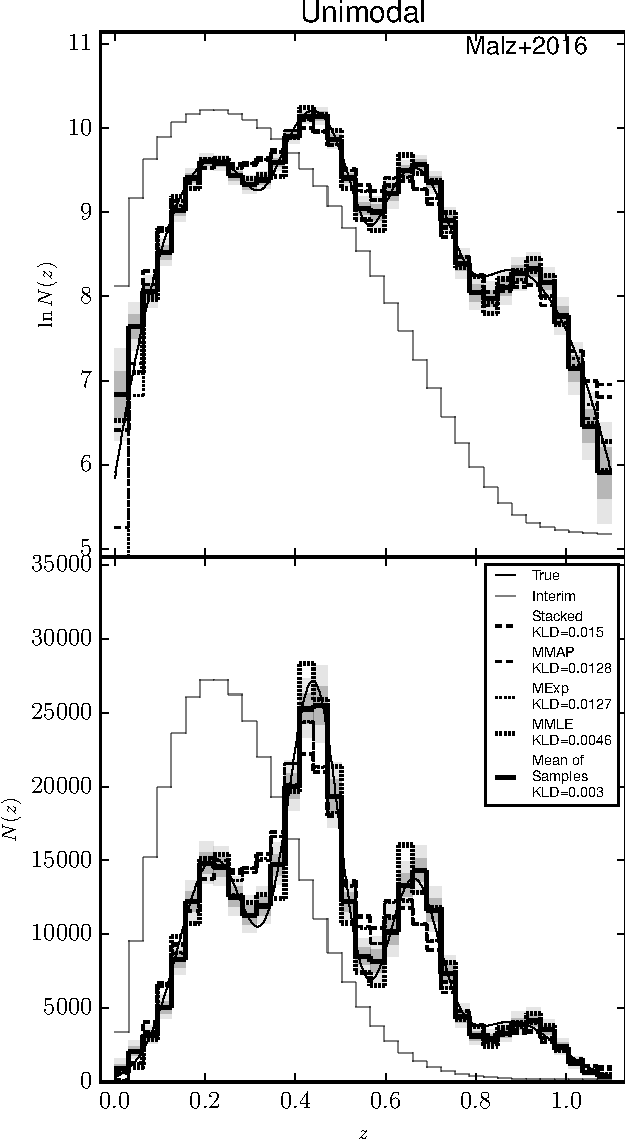
\includegraphics[width=0.5\textwidth]{figs/uint/comps.pdf}
\caption{The interim prior (gray line) is biased towards lower redshifts.  The 
mean of the sampled values (thick, solid line; KLD $0.002$) and marginalized 
MLE (thick, dotted line; KLD $0.003$) are unaffected by the nontrivial interim 
prior, taking the same KLD values as in the fiducial case with a flat interim 
prior.  However, the alternatives yield biased estimates, both smoothing the 
features of the true $N(z)$ (thin, solid line) and showing a bias to low 
redshift values according to the interim prior.  Stacking (thick, dashed line; 
KLD $0.017$) does the worst of the three alternatives, with the marginalized 
MAP (thin, dashed line; KLD $0.015$) and marginalized expected value (thin, 
dotted line; KLD $0.014$) doing slightly better.}
\label{fig:intu-comp}
\end{figure}


Fig. \ref{fig:intb-comp} shows the comparison of the mean of the sample values 
to the true values and the result of stacking.  What is most striking is that 
stacking is very strongly affected by the choice of the interim prior, whereas 
the mean of the samples is only weakly affected by it and the marginalized MLE 
is not affected by it very much at all.  Based on these results, it can be 
concluded that when the interim prior is known to be inappropriate, the 
marginalized MLE is the best estimator of the truth.  

%\begin{figure}
%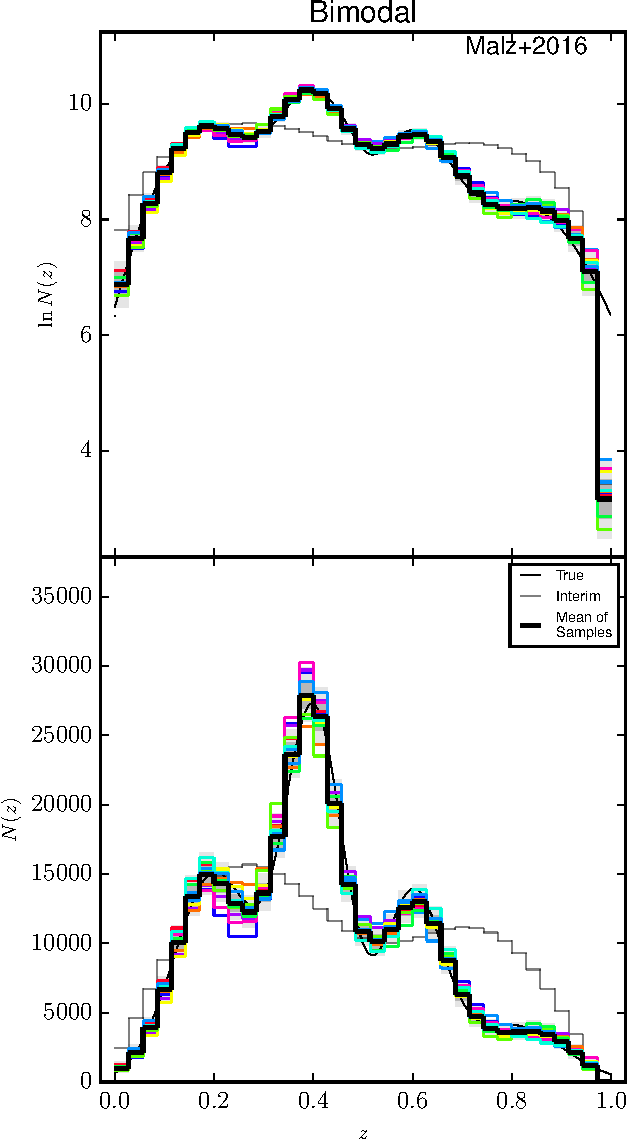
\includegraphics[width=0.5\textwidth]{figs/bint/samps.pdf}
%\caption{The mean (thick, black line) of the samples (colored lines) show some 
%influence of the interim prior (gray line) but also replicate some of the featu
%res of the true $N(z)$ (thin, black line).}
%\label{fig:intb-samp}
%\end{figure}

\begin{figure}
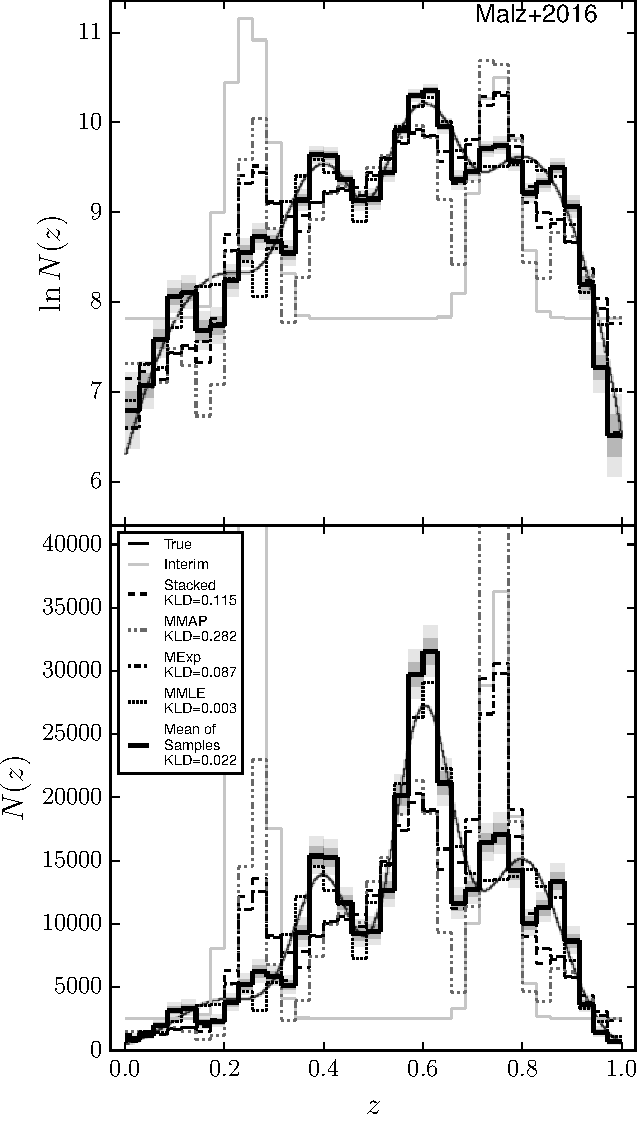
\includegraphics[width=0.5\textwidth]{figs/bint/comps.pdf}
\caption{The interim prior (gray line) is biased toward low and high redshifts. 
 In this case, the marginalized MLE (thick, dotted line; KLD $0.003$) best 
recovers the true $N(z)$ (thin, solid line), with the mean of samples (thick, 
solid line; KLD $0.005$) as a close second.  The point estimators and stacking 
have comparable results, with the marginalized MAP (thin, dashed line; KLE 
$0.01$) being the best of them and the marginalized expected value (thin, 
dotted line) and stacked result (thick, dashed line) sharing the same KLD of 
$0.012$.}
\label{fig:intb-comp}
\end{figure}

%\clearpage
\subsection{Data}
\label{sec:boss}

The results of the inference are shown in Figs. \ref{fig:dataparam} and 
\ref{fig:datacomp}.  

\begin{figure}
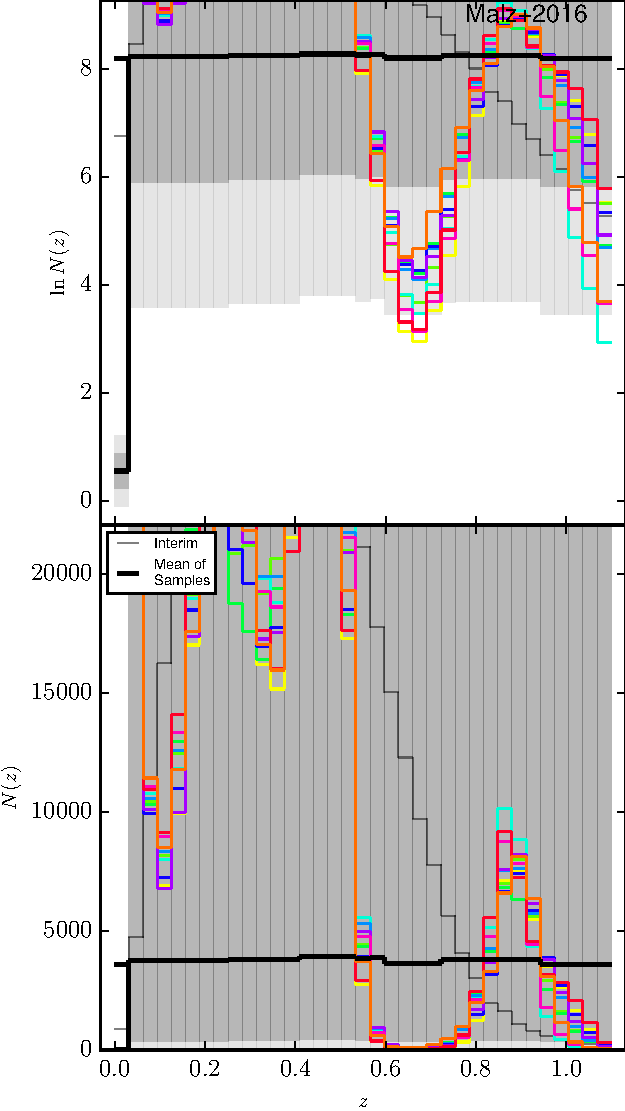
\includegraphics[width=0.5\textwidth]{figs/boss/samps.pdf}
\caption{Samples from the full posterior (colored lines) of the subsample 
differ substantially from the interim prior (gray).  The mean of samples 
(thick, black line) and associated error bars ($1\sigma$ in dark gray, 
$2\sigma$ in light gray) are in line with the sampled values.}
\label{fig:dataparam}
\end{figure}

\begin{figure}
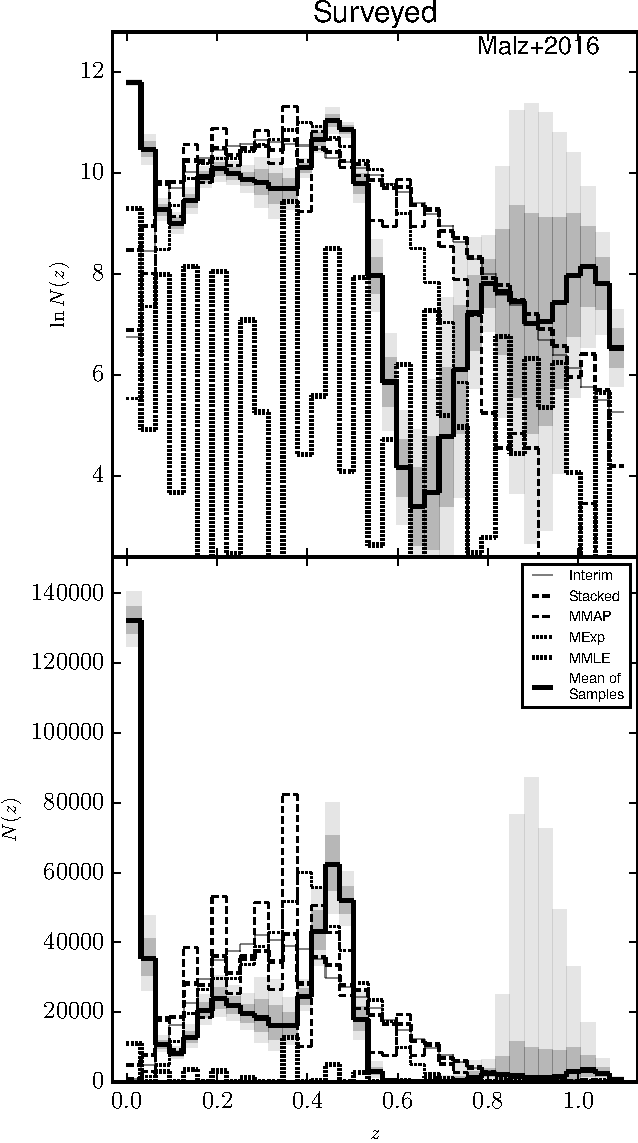
\includegraphics[width=0.5\textwidth]{figs/boss/comps.pdf}
\caption{The results of each of several estimators are shown here.  It can be 
seen that stacking (thick, dashed line) and the point estimators (marginalized 
MAP as thin, dashed line; marginalized expected value as thin, dotted line) 
yield a broader distribution with fewer features, closely matching the interim 
prior (gray, solid line) than the mean of the samples (thick, solid line).  The 
marginalized MLE (thick, dotted line) is highly unstable, as was true in the 
simulated case with multimodal photo-$z$ likelihoods that more closely 
resembled the data of this case.}
\label{fig:datacomp}
\end{figure}

It is worth discussing two systematic effects evident in the results.  Because 
the data itself exhibits high uncertainty at high $z$ in the form of local 
maxima of the photo-$z$ interim posteriors, a reflection of the inherent 
degeneracies that give rise to catastrophic photo-$z$ errors, it is natural 
that there be large errors in that region.  Another effect worth investigating 
is the instability of the marginalized maximum likelihood estimator.  
\textbf{I'm not sure how to justify my explanation that the MMLE fails more 
severely on more strongly multimodal data without showing the results of the 
tests that proved it.}

The BOSS subsample is further subsampled by imposing a cut in $r$-band 
magnitude (at the median magnitude) to approximate the behavior of a heavily 
biased galaxy survey with a magnitude limit.  Samples of photo-$z$ interim 
posteriors are shown in the right panel of Fig. \ref{fig:datapzs}.  The results 
of the inference are shown in Figs. \ref{fig:biasparam} and \ref{fig:biascomp}. 
 

\begin{figure}
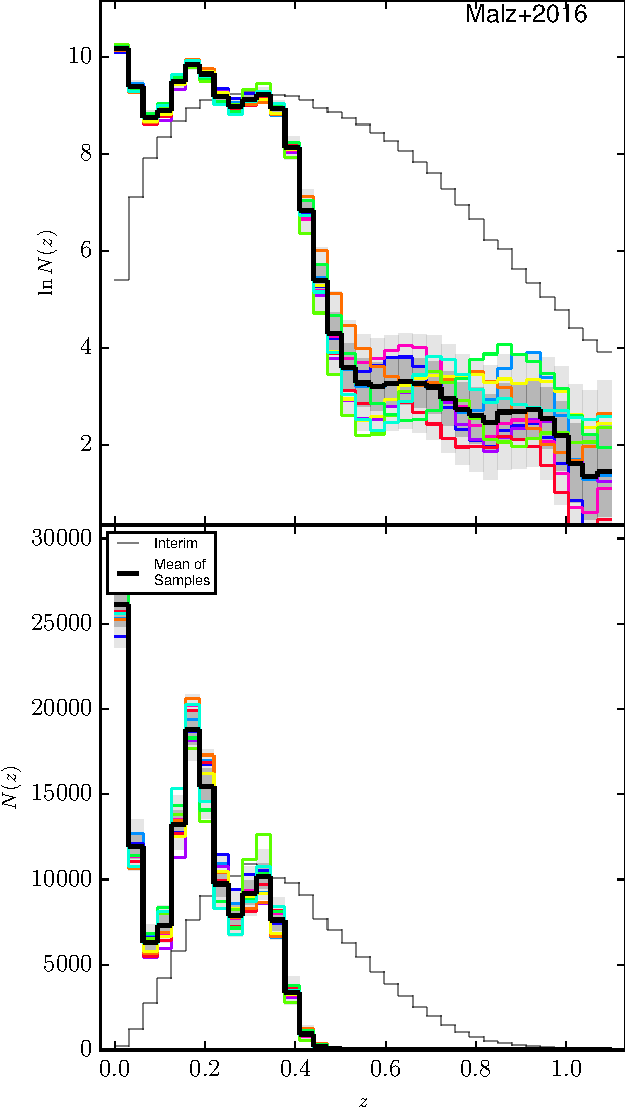
\includegraphics[width=0.5\textwidth]{figs/bias/samps.pdf}
\caption{Samples from the full posterior (colored lines) of the biased 
subsample differ substantially from the interim prior (gray).  The mean of 
samples (thick, black line) and associated error bars ($1\sigma$ in dark gray, 
$2\sigma$ in light gray) are in line with the sampled values.}
\label{fig:biasparam}
\end{figure}

\begin{figure}
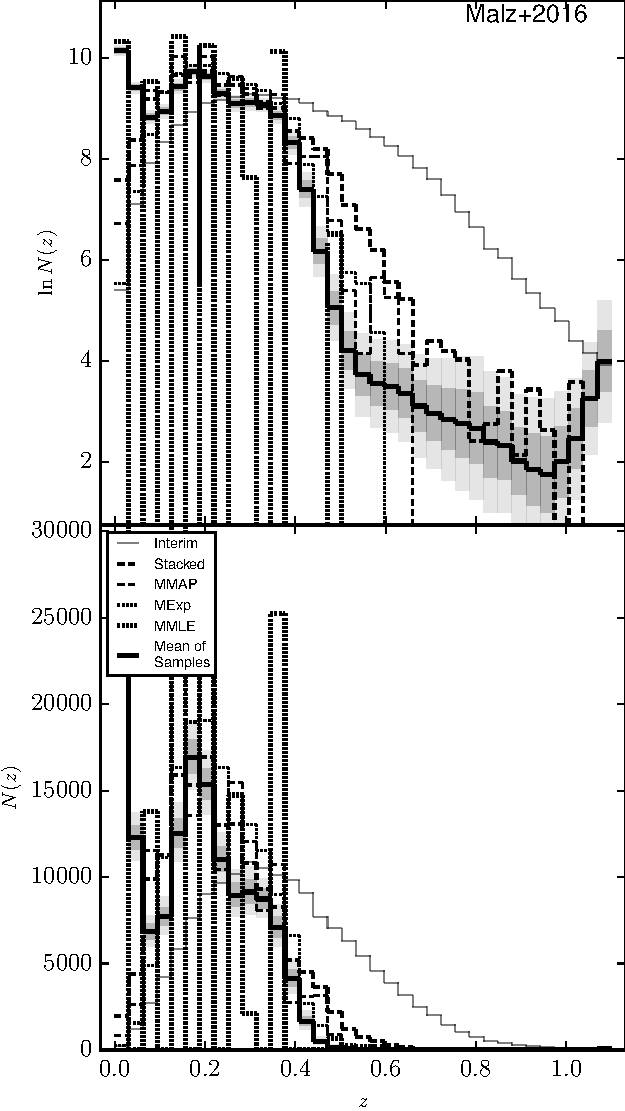
\includegraphics[width=0.5\textwidth]{figs/bias/comps.pdf}
\caption{The results of each of several estimators are shown here.  First, it 
should be noted that the interim prior (gray, solid line) differs substantially 
from all the estimators.  Second, it can be seen that stacking (thick, dashed 
line) estimates a broader distribution with fewer features than the mean of the 
samples (thick, solid line).  The marginalized MLE (thick, dotted line) is 
highly unstable, as was true in the simulated case with multimodal photo-$z$ 
likelihoods that more closely resembled the data.}
\label{fig:biascomp}
\end{figure}

One can note that in these figures, the large error bars at high $z$ are 
reduced to the size of those at lower redshifts.  Because the cut in magnitude 
eliminates the dimmest galaxies for which redshifts cannot be well constrained, 
the interim photo-$z$ posteriors that had local maxima at those redshifts are 
not included in the sample.  Nonetheless, the marginalized MLE is still 
unstable, although not as much as in the case of unbiased pseudo-random data.  
The instability is due to the fact that the photo-$z$ interim posteriors are 
still highly multimodal, but the improved agreement with the other methods is 
due to the fact that they are less so than in the unbiased case.

%\clearpage
\section{Conclusion}
\label{sec:con}

This study derives and demonstrates a mathematically consistent implementation 
of inference of a one-point statistic based on interim photo-$z$ posteriors.  
The fully Bayesian method, based in the fundamental laws of probability, begins 
with a graphical model corresponding to equations for the full posterior.  The 
technique developed in this paper is applied to the example of the redshift 
distribution function $N(z)$ with promising results on mock data; not only is 
this the only mathematically correct approach to the problem, it also recovers 
the true parameter values better than popular alternatives.  

In the tests on simulated data performed here, the full posterior distribution 
over the hyperparameters defining $N(z)$ derived by this method is consistent 
with the true hyperparameter values, making the mean of sampled values an 
excellent estimator of $N(z)$.  The results of those tests is summarized below 
and in Tab. \ref{tab:kld}, where lower values indicate a closer match between 
the true $N(z)$ and the estimator.  Tests were performed on subsets of BOSS 
data with results consistent with those of simulations.

\begin{enumerate}
\item Both the marginalized MLE and the mean of the samples are good estimators 
of $N(z)$ for the simplest photo-$z$ posteriors.
\item When data suffers from imprecision, as in the case of high intrinsic 
scatter, the difference between stacking and sampling is highly pronounced, 
with stacking yielding a much smoother estimator of $N(z)$ and sampling 
producing a broader posterior with the same mean hyperparameter values as in 
the case of cleaner data.
\item When data suffers from inaccuracies, as in the case of catastrophic 
outliers, the marginalized MLE is unstable, point estimators are subject to 
catastrophic errors, and stacking yields an especially smoothed estimate of 
$N(z)$; sampling does the best job of recovering the true $N(z)$, but it does 
not do as well as in cases where the generative model reflected in the full 
likelihood matches the way the data were produced.
\item The marginalized MLE is an excellent estimator for strongly featured 
$N(z)$ with simple, clean photo-$z$ posteriors; stacking smooths features more 
than sampling and photo-$z$ point estimation.
\item When the interim prior is known to be a poor approximation to the data, 
only the marginalized MLE and mean of sampled values are satisfactory 
estimators of $N(z)$ because they are the only methods that can account for the 
bias introduced into the photo-$z$ posteriors; this is the most compelling case 
because of the ubiquity of using inappropriate interim priors.
\end{enumerate}

\begin{table}
\begin{tabular}{lccccc}
& Mean of & Marginalized & Stacking & Marginalized & Marginalized\\
& Samples & MLE & & MAP & Expected Value\\
Fiducial &&&&&\\
2xImprecise &&&&&\\
4xImprecise &&&&&\\
Inaccurate &&&&&\\
Multimodal &&&&&\\
Featured &&&&&\\
Unimodal &&&&&\\
Bimodal &&&&&
\end{tabular}
\caption{The best-fit estimator in each case is bolded.  \textbf{This table 
will be filled in once I'm certain I won't be re-running any tests.}}
\label{tab:kld}
\end{table}

By showing that this method is effective in recovering the true redshift 
distribution function and posterior distributions on its parameters from 
simulated interim photo-$z$ posteriors, this work supports the production of 
interim photo-$z$ posteriors by upcoming photometric surveys such as LSST so 
that more accurate inference of physical parameters may be accessible to the 
scientific community.  We discourage researchers from co-adding interim 
photo-$z$ posteriors or converting them into point estimates of redshift and 
instead recommend the use of Bayesian probability to guide the usage of interim 
photo-$z$ posteriors in science.  We emphasize to those who produce interim 
photo-$z$ posteriors from data that it is essential to release the interim 
prior used in generating this data product in order for proper inference to be 
conducted by consumers of this information.

The method herein developed is applicable with minimal modification to other 
one-point statistics of redshift to which we will apply this method in the 
future, such as the redshift-dependent luminosity function and weak lensing 
mean distance ratio.  Future work will also include the extension of this fully 
probabilistic approach to higher-order statistics of redshift such as the 
two-point correlation function.

\textbf{What else should I be putting here?  Is this too terse?}

%\clearpage

\begin{acknowledgements}
AIM thanks Mohammadjavad Vakili for insightful input on statistics and Boris 
Leistedt for helpful comments provided in the preparation of this paper.
\end{acknowledgements}

\textbf{Let me know if anything is screwed up with my references; I made a mess 
wrestling with Mendeley and BibDesk and may have missed something when cleaning 
up.}
\bibliographystyle{apj}
\bibliography{zPDF}

\end{document}